\documentclass{report}

% Packages for math symbols and equations
\usepackage[T1]{fontenc}
\usepackage[utf8]{inputenc}

\usepackage[margin=1.4in]{geometry}
\usepackage{graphicx}

\usepackage{amssymb,amsthm, amsmath}
%\usepackage{mathtools}
%\numberwithin{equation}{section}

\usepackage[
natbib,
style=alphabetic,
maxbibnames=10,  
sorting=ydnt,
url=false,
doi=false,
sortcites,
defernumbers,
backref,
backend=biber
]{biblatex}
\addbibresource{bibliography.bib}

\usepackage{hyperref}

\usepackage{todonotes}
%\setuptodonotes{inline}
\usepackage{url}

\usepackage[nameinlink, capitalise, noabbrev]{cleveref}

\usepackage{xfrac}
\usepackage{nicefrac}

\usepackage{soul}

\usepackage{bbm}

\usepackage{enumitem}

%For double brackets \llbracket \rrbracket
\usepackage{stmaryrd}

\crefname{assumption}{Assumption}{Assumptions}

\newtheorem{theorem}{Theorem}

\newtheorem{proposition}{Proposition}[section]
\newtheorem{lemma}{Lemma}[section]
\newtheorem{corollary}{Corollary}[section]
\theoremstyle{remark}
\newtheorem{remark}{Remark}[section]


\theoremstyle{definition}
\newtheorem{example}{Example}[section]
\newtheorem{counterexample}{Counterexample}[section]
\newtheorem{definition}{Definition}[section]
\newtheorem{assumption}{Assumption}
\newtheorem{question}{Question}
\newtheorem{exercise}{Exercise}
\newtheorem{fact}{Fun Fact}
%\numberwithin{equation}{section}

%\renewcommand{\baselinestretch}{2}

%\newcounter{hypcounter}

\newcommand{\N}{\mathbb{N}}
\newcommand{\Z}{\mathbb{Z}}
\newcommand{\R}{\mathbb{R}}
%\DeclareMathOperator{\dom}{dom}
\newcommand{\closure}[1]{\overline{#1}}
\newcommand{\norm}[1]{\left\Vert #1 \right\Vert}
\newcommand{\seminorm}[1]{\left[ #1 \right]}
\newcommand{\abs}[1]{\left\vert #1 \right\vert}
%\DeclareMathOperator{\divtmp}{div}
\renewcommand{\div}{\divtmp}
% \DeclareMathOperator{\argmin}{arg\,min}
% \DeclareMathOperator{\argmax}{arg\,max}
% \DeclareMathOperator{\esssup}{ess\,sup}
% \DeclareMathOperator{\essinf}{ess\,inf}
\renewcommand{\st}{\,:\,}
% \DeclareMathOperator{\supp}{supp}
\newcommand{\dx}{\,\mathrm{d}x}
\renewcommand{\d}{\,\mathrm{d}}
\newcommand{\dH}{\,\mathrm{d}\mathcal{H}^{n-1}(x)}
% \DeclareMathOperator{\sign}{sign}
\newcommand{\eps}{\varepsilon}
% \DeclareMathOperator{\dist}{dist}
% \DeclareMathOperator{\Lip}{Lip}
\newcommand{\KR}{\mathrm{KR}}
\newcommand{\C}{\mathrm{C}}
\renewcommand{\L}{\mathrm{L}}
\newcommand{\W}{\mathrm{W}}
\newcommand{\M}{\mathcal M}
\newcommand{\grad}{\nabla}
\newcommand{\hess}{\mathrm{D}^2}
\newcommand{\defeq}{:=}
% \DeclareMathOperator{\diam}{diam}
\newcommand{\Set}[1]{\left\lbrace#1\right\rbrace}
\newcommand{\scale}{\eps}
\newcommand{\res}{\delta}


\newcommand{\wto}{\rightharpoonup}
\newcommand{\wsto}{\overset{\ast}{\rightharpoonup}}
\newcommand{\strictto}{\overset{\mathrm{str}}{\rightharpoonup}}

\newcommand{\rev}{\color{magenta}}
\renewcommand{\rev}{}
\newcommand{\red}{\color{red}}
\newcommand{\blue}{\color{blue}}
\newcommand{\nc}{\normalcolor}


% Lie math operators
\DeclareMathOperator{\toledo}{T}
\DeclareMathOperator{\isom}{Isom}
\DeclareMathOperator{\bus}{b}
\DeclareMathOperator{\ii}{i}
\DeclareMathOperator{\spa}{span}
\DeclareMathOperator{\class}{C}
\DeclareMathOperator{\diam}{diam}
\DeclareMathOperator{\diag}{diag}
\DeclareMathOperator{\U}{{\mathrm{U}}}
\DeclareMathOperator{\SL}{{\mathrm{SL}}}
\DeclareMathOperator{\ssl}{{\mathfrak{sl}}}
\DeclareMathOperator{\SU}{{\mathrm{SU}}}
\DeclareMathOperator{\Sp}{{\mathrm{Sp}}}
\DeclareMathOperator{\ssp}{{\mathfrak{sp}}}
\DeclareMathOperator{\su}{{\mathfrak{su}}}
\DeclareMathOperator{\PSL}{{\mathrm{PSL}}}
\DeclareMathOperator{\GL}{{\mathrm{GL}}}
\DeclareMathOperator{\gl}{{\mathfrak{gl}}}
\DeclareMathOperator{\SO}{{\mathrm{SO}}}
\DeclareMathOperator{\sso}{{\mathfrak{so}}}
\DeclareMathOperator{\PGL}{{\mathrm{PGL}}}
\DeclareMathOperator{\PO}{{\mathrm{PO}}}
\DeclareMathOperator{\PSO}{{\mathrm{PSO}}}
\DeclareMathOperator{\im}{{\mathrm{Im}}}
\DeclareMathOperator{\id}{id}
\DeclareMathOperator{\inte}{int}
\DeclareMathOperator{\LC}{LC{}}
\DeclareMathOperator{\F}{Frenet{}}
\DeclareMathOperator{\lie}{Lie}
\DeclareMathOperator{\Ker}{Ker}
\DeclareMathOperator{\Ad}{Ad}
\DeclareMathOperator{\ad}{ad}
\DeclareMathOperator{\Hff}{dim_{Hf{}f}}
\DeclareMathOperator{\vol}{Vol}
\DeclareMathOperator{\rk}{rank}
%\DeclareMathOperator{\jac}{jac}
\DeclareMathOperator{\gap}{{\sf{gap}}}
\DeclareMathOperator{\ann}{Ann}
\DeclareMathOperator{\tr}{tr}
\DeclareMathOperator{\rad}{rad}
\DeclareMathOperator{\Sym}{Sym}

%:= sign
\newcommand{\equaldef}{\overset{\mathrm{def}}{=}}

\newcommand{\restr}{\mathbin{\vrule height 1.6ex depth 0pt width
0.13ex\vrule height 0.13ex depth 0pt width 1.3ex}}

\usepackage{tikz-cd}


% Title page information
\title{Lie group notes}
\author{Giorgos}
\date{\today}

\begin{document}

\maketitle

\tableofcontents

\chapter*{Conventions}
\begin{itemize}
    \item By Lie group, we mean either real or complex.
    \item A closed Lie subgroup of a Lie group is a submanifold that is also a subgroup (see \cref{thm:closed_subgroup}). 
    \item A Lie subgroup is a subgroup that is also an immersed submanifold.
\end{itemize}

\chapter{Lie groups: basic definitions}
We will have two notions of subgroups of Lie groups:
\begin{definition}
    Let $G$ be a complex or real Lie group and $H$ be a subgroup of $G$.
    \begin{enumerate}[label = (\roman*)]
        \item $H$ is a Lie subgroup if it is an immersed submanifold of $G$ with the multiplication and inverse maps being smooth (or analytic).
        \item $H$ is a closed Lie subgroup if it is an embedded submanifold of $G$.
    \end{enumerate}
\end{definition}
\begin{example}
    Any of the classical Lie groups are closed Lie subgroups of $\GL(n, \mathbb K)$.
    For a Lie subgroup that is not closed, consider the irrational winding on the torus, that is $G = \mathbb T^2 = \mathbb R^2/\mathbb Z^2$, and $H = f(\mathbb R)$ with $f(t,s) = (t \mod \mathbb Z, \alpha s \mod \mathbb Z)$, where $\alpha \in \mathbb R\backslash \mathbb Q$.
\end{example}
\section{Lie subgroups and quotients}
The following theorem allows us to reduce the study of Lie groups to the study of finite groups and connected Lie groups, since $G_0$ is a normal subgroup of $G$ and $G/G_0$ is a discrete group.
where $G^0$ is the identity component of $G$.
\begin{theorem}[Theorem 2.6, \cite{kirillov2008introduction}]
    Let $G$ be a real or complex Lie group and $G^0$ its identity component.
    Then $G^0$ is a normal subgroup of $G$ and a Lie group itself, while $G/G^0$ is a discrete group.
\end{theorem}

In fact, we can reduce the case of connected Lie groups to simply connected Lie groups:
\begin{theorem}[Theorem 2.7, \cite{kirillov2008introduction}]
    Let $G$ be a connected Lie group. Then its universal cover $\tilde G$ has a canonical structure of a Lie group such that the covering map $p: \tilde G \to G$ is a homomorphism of Lie groups whose kernel is isomorphic to the fundamental group of $G$.
    Moreover, in this case, $\ker p$ is a discrete central subgroup in $\tilde G$.
\end{theorem}
\begin{proof}
    The lifting property of the universal cover implies that $\tilde G$ is a Lie group.
    The kernel is discrete, being the fiber of a covering map.
    The fact that it is central follows from the more general fact that every discrete normal subgroup of a connected Lie group is central.
    To show the latter, one considers the map $G \to N, g \to g n g^{-1}$ where $N$ is the normal subgroup and $n \in N$ is some fixed element.
    Then the inverse image of any element $n' \in N$ is closed an open in $G$, so it is all of $G$ in the case where $n' = n$ and empty otherwise.
\end{proof}

\begin{example}
    In the case where $G = \mathbb T^2$ is the torus, the covering map $p: \mathbb R^2 \to \mathbb T^2$ is given by $p(t,s) = e^{2\pi i t, 2\pi i s }$, and $\ker p = \mathbb N^2 \simeq \pi_1(\mathbb T^2)$.
\end{example}

We have the following connection between subgroups and Lie subgroups (i.e.\ subgroups that are also submanifolds):
\begin{theorem}[Theorem 2.8, \cite{kirillov2008introduction}]\label{thm:closed_subgroup}
    \begin{enumerate}[label=(\roman*)]
        \item Any Lie subgroup of a Lie group is closed in the topology of the ambient group.
        \item Any closed subgroup of a Lie group is a real Lie subgroup.
    \end{enumerate}
\end{theorem}
\begin{proof}
    For the first part of the theorem, we note that $\overline H$ is a subgroup of $G$ as well.
    We claim that $H$ (and thus $Hx$ for every $x \in \overline H$ ) is open and dense in $\overline H$.
    To see this, note that $e \in \overline H$ implies that for every neighborhood $U \subseteq G$ of $e$ in $G$, $U \cap H$ is nonempty.
    In particular there exists some open set $U$ in $G$ containing $r$ such that $U \cap H \neq \emptyset$.
    Then $U\cap H$ will be a neighborhood of $e$ in $\overline H$ and $H$ is open because it can be written as the union of all subsets of the form $h(U\cap H)$ for $h \in H$.

    To conclude, note that for $x, y \in \overline H$, $Hx \cap Hy$ is dense in $\overline H$, so it is nonempty.
    This implies that $Hx = Hy = H$ and $H$ thus $H = \overline H$.
\end{proof}
\section{Homogeneous spaces}
We begin by describing coset spaces of Lie groups.
\begin{theorem}[Theorem 2.11, \cite{kirillov2008introduction}]
    Let $G$ be a Lie group of dimension $n$, $H \leq G$ a closed Lie subgroup of dimension $k$.
    \begin{enumerate}[label = (\roman*)]
        \item The coset space $G/H$ has a natural structure of a manifold of dimension $n-k$ such that the canonical map $p: G \to G/H$ is a fiber bundle, with fiber diffeomorphic to $H$.
        The tangent space at the identity is isomorphic to the quotient space $T_H G/H \simeq T_eG/T_eH$.
        \item If H is a normal closed Lie subgroup then $G/H$ has a canonical Lie group structure.
    \end{enumerate}
\end{theorem}

The following is the analog of the homomorphism theorem for Lie groups:
\begin{theorem}[Theorem 2.5, \cite{kirillov2008introduction}]
    Let $f:G_1 \to G_2$ be a Lie group morphism.
    \begin{enumerate}[label = (\roman*)]
        \item $H = \ker f$ is a normal closed Lie subgroup of $G_1$ and $f$ induces an injective homomorphism $G_1/H \to G_2$ that is an immersion
        \item If moreover $\Im f$ is an embedded submanifold, then it is a closed Lie subgroup of $G_2$ and $f$ induces an isomorphism $G_1/H \to \Im f$.
    \end{enumerate}
\end{theorem}


\begin{theorem}[Theorem 2.20, \cite{kirillov2008introduction}]
    Let $G$ be a Lie group acting on a manifold $M$, and $m \in M$.
    \begin{enumerate}[label = (\roman*)]
        \item The stabilizer $G_m$ is a closed Lie subgroup of $G$, with Lie algebra
        \[
        \mathfrak h = \{ x \in \mathfrak g \mid \rho_*(x)(m) = 0 \}.
        \]
        where $\rho: G \to \mathrm{Diff}(M)$ is the action of $G$ on $M$.
        \item The orbit map $g \mapsto g \cdot m$ induces an injective immersion $G/G_m \hookrightarrow \mathcal O_m$ whose image coincides with $\mathcal O_m$.
        \item The orbit $\mathcal O_m$ is an immersed submanifold with tangent space $T_m \mathcal O_m = \mathfrak g / \mathfrak h $.
        \item If the orbit is a submanifold, then the orbit map is a diffeomorphism.
    \end{enumerate}
\end{theorem}
\begin{proof}
See \cite[Theorem 2.20, Theorem 3.29]{kirillov2008introduction}.
\end{proof}

The case of one orbit gives rise to $G$-homogeneous spaces:
\begin{theorem}[Theorem 2.22 \cite{kirillov2008introduction}]
    Let $M$ be a $G$-homogeneous space and $m \in M$.
    Then the orbit map $G \to M$ is a fiber bundle over $M$ with fiber $G_m$.
\end{theorem}

The following proposition gives us a way to check whether a Lie group morphism is a covering map:
\begin{proposition}[Lie morphism covering map criterion]
    Let $f:G_1 \to G_2$ be a Lie group morphism such that $f_*: \mathfrak g_1 \to \mathfrak g_2$ is an isomorphism.
    Then $f$ is a covering map and $\ker f$ is a discrete central group.
\end{proposition}
\begin{proof}
    The inverse mapping theorem tells us that there exist neighborhoods $U_1, U_2$ of the identities of $G_1$ and $G_2$ respectively such that $f:U_1 \to U_2$ is a diffeomorphism.
    In particular, $f$ is surjective since its image contains $U_2$ which generates $G_2$, being a neighborhood of the identity.
    Moreover, for every $g \in G_1$ and $z_1, z_2 \in \ker f$:
    \[
        gU_1 z_1 \cap gU_2 z_2 = \{e_1\} \text{ unless } z_1 = z_2.
    \]
    Indeed, if $g u z_1 = g v z_2$ for some $u, v \in U$, then $u = v z_2 z_1^{-1}$, so $f(u) = f(v)$.
    But $f$ being injective on $U_1$, this implies $u = v$ and $z_1 = z_2$.

    Thus $f(g)U_1$ is an evenly covered neighborhood for every $f(g) \in G_2$.
    \[
    f^{-1}(f(g)U_2) = g U_1 \ker f = \bigsqcup_{z \in \ker f} g U_1 z.
    \]

    To see that $\ker f$ is discrete, note that the injectivity of $f$ implies $U_1 \cap \ker f = \{ e_1 \}$.
    Being a discrete normal subgroup, it must also be central.
\end{proof}

\section{Classical Lie groups}

\begin{definition}
    We define
    \[
    Sp(n, \mathbb K) = 
    \left\{
        A \in GL(2n, \mathbb K) \mid \omega(Ax, Ay) = \omega(x, y)
    \right\}.
    \]
    where $\omega$ is the standard symplectic form on $\mathbb K^{2n}$, which is given by
    $\omega(x, y) = x^* J y = \sum_{i=1}^n x_i y_{i+n} - x_{i+n}y_i$, 
    and 
    \[
    J = 
    \begin{pmatrix}
    0 & -I_n \\
    I_n & 0
    \end{pmatrix}.
    \]
    We also define the gorup of unitary quaternionic transformations by
    \[
    \Sp(n) = \Sp(n, \mathbb C) \cap \SU(2n).
    \]
\end{definition}

The following theorem tells us that the logarithmic map behaves well when restricted to a neighborhood of the identity in each classical group.

\begin{table}[h!]
    \centering
    \begin{tabular}{c c c c c c}
        $G$ & $O(n, \mathbb{R})$ & $SO(n, \mathbb{R})$ & $U(n)$ & $SU(n)$ & $Sp(n)$ \\
        \hline \hline
        $\mathfrak{g}$ & $x^t = -x$ & $x^t = -x$ & $x^* = -x$ & $x^* = -x, \ \text{tr}, x = 0$ & $J^{-1}x^*J = -x, x^* = -x$ \\
        $\dim G$ & $\frac{n(n-1)}{2}$ & $\frac{n(n-1)}{2}$ & $n^2$ & $n^2 - 1$ & $n(2n+1)$ \\
        $\pi_0(G)$ & $\mathbb{Z}_2$ & $\{1\}$ & $\{1\}$ & $\{1\}$ & $\{1\}$ \\
        $\pi_1(G)$ & $\mathbb{Z}_2 \ (n \ge 3)$ & $\mathbb{Z}_2 \ (n \ge 3)$ & $\mathbb{Z}$ & $\{1\}$ & $\{1\}$ \\
        $\mathfrak{g}_{\mathbb C}$ &  &  & $\mathfrak{gl}(n, \mathbb C)$ & $\mathfrak{sl}(n, \mathbb C)$ & 
    \end{tabular}
    \caption{Compact classical groups}
    \label{table:classical_groups}
\end{table}

\begin{table}[h!]
    \centering
    \begin{tabular}{c c c c}
        $G$ & $GL(n, \mathbb{R})$ & $SL(n, \mathbb{R})$ & $Sp(n, \mathbb{R})$ \\
        \hline \hline
        $\mathfrak{g}$ & $\mathfrak{gl}(n, \mathbb{R})$ & $\text{tr} \, x = 0$ & $x + J^{-1}x'J = 0$ \\
        $\dim G$ & $n^2$ & $n^2 - 1$ & $n(2n + 1)$ \\
        $\pi_0(G)$ & $\mathbb{Z}_2$ & $\{1\}$ & $\{1\}$ \\
        $\pi_1(G)$ & $\mathbb{Z}_2 \ (n \ge 3)$ & $\mathbb{Z}_2 \ (n \ge 3)$ & $\mathbb{Z}$ \\
        $\mathfrak{g}_{\mathbb C}$ &  & $\mathfrak{sl(n, \mathbb C)}$ &  
    \end{tabular}
    \caption{Noncompact real classical groups.}
    \label{table:noncompact_real_classical_groups}
\end{table}

\begin{table}[h!]
    \centering
    \begin{tabular}{c c c c c}
        $G$ & $GL(n, \mathbb{C})$ & $SL(n, \mathbb{C})$ & $O(n, \mathbb{C})$ & $SO(n, \mathbb{C})$ \\
        \hline \hline
        $\pi_0(G)$ & $\{1\}$ & $\{1\}$ & $\mathbb{Z}_2$ & $\{1\}$ \\
        $\pi_1(G)$ & $\mathbb{Z}$ & $\{1\}$ & $\mathbb{Z}_2$ & $\mathbb{Z}_2$ \\
    \end{tabular}
    \caption{Complex classical groups.}
    \label{table:complex_classical_groups}
\end{table}

\chapter{Lie groups and Lie algebras}
\section{Exponential map}
\begin{definition}[Proposition 3.1, \cite{kirillov2008introduction}]
    Let $G$ be a Lie group and $x \in \mathfrak g$.
    The one-parameter subgroup $\gamma_x: \mathbb K \to G$ is the unique Lie group morphism such that $\gamma_x'(0) = x$.
    We define the exponential map of $G$ as
    \[
    \exp(x) = \gamma_x(1)
    \]
\end{definition}
\begin{remark}
    By looking at the proof of the statements in the above definition, one can see that for $x\in \mathfrak g$, the curve
    \[
    \exp(tx) = \gamma_x(t) = \gamma_{tx}(1).
    \]
    integral curve of the left-invariant vector field $X \in \mathcal X(G)$ that satisfies
    \[
    X_e = x.
    \]
\end{remark}

The following are some properties of the exponential map:
\begin{theorem}[Theorems 3.7 and 3.36, \cite{kirillov2008introduction}]
    Let $G$ be a Lie group.
    \begin{enumerate}[label = (\roman*)]
        \item $d_{e} \exp = \id_{\mathfrak g}$
        \item The exponential map is a local diffeomorphism at $0$.
        \item For any Lie group morphism $\phi:G_1 \to G_2$, we have $d_e \phi (exp(x)) = \exp d_e (\phi(x))$ for all $x\in \mathfrak g$.
        \item For any $g \in G, x \in \mathfrak g$
        \[
        g \exp(x) g^{-1} = \exp(\Ad_g x).
        \]
        \item For $x, y \in \mathfrak g$, we have:
        \[
        \text{If } [x,y] = 0 \text{ then } e^x e^y = e^y e^x = e^{x+y}.
        \]
    \end{enumerate}
\end{theorem}

\begin{remark}
    The exponential map is not surjective in general. It is however for compact Lie groups.
\end{remark}

\begin{lemma}
    The exponential map of a connected Lie group $G$ sends generators of $\mathcal g$ to generators of $G$.
    That is, if $\{ x_1, \ldots, x_n \}$ is a basis of $\mathfrak g$, then $\left\{ \exp(t x_i) : t \in \mathbb R, i \in \llbracket 1, n \rrbracket \right\}$ is a basis of $G$.
\end{lemma}
\begin{proof}
    Consider the map $f: \mathbb R^n \to \mathbb G$ given by
    \[
    f(t_1, \ldots, t_n) = \exp(t_1 x_1) \cdots \exp(t_n x_n).
    \]
    Then $d_0 f = I_n$ in the basis with respect to the standard basis for $\mathbb R^n$ and $\{ x_1, \ldots, x_n \}$ for $\mathfrak g$.
    In particular it is surjective and by the constant rank theorem, $f(\mathbb R^n)$ contatins a neighborhood of the identity of $G$. 
\end{proof}
\begin{example}
    Let $G = SO(3, \mathbb R)$.
    Then $\mathfrak{so}(3, \mathbb R)$ consists of skew-symmetric mattrices, with basis:
    \begin{align*}
        J_1 = \begin{pmatrix} 0 & 0 & 0 \\ 0 & 0 & -1 \\ 0 & 1 & 0 \end{pmatrix}, \quad
        J_2 = \begin{pmatrix} 0 & 0 & 1 \\ 0 & 0 & 0 \\ -1 & 0 & 0 \end{pmatrix}, \quad
        J_3 = \begin{pmatrix} 0 & -1 & 0 \\ 1 & 0 & 0 \\ 0 & 0 & 0 \end{pmatrix}.
    \end{align*}
    The exponential matrix is given by
    \[
    e^{tJ_1} = 
    \begin{pmatrix}
        1 & 0 & 0 \\
        0 & \cos(t) & -\sin(t) \\
        0 & \sin(t) & \cos(t)
    \end{pmatrix},
    \]
    i.e.\ rotation around x-axis by angle t; similarly, $J_y, J_z$ generate rotations around
    $y, z$ axes.
    Elements of the form $exp(tJx), exp(tJ_y ), exp(tJ_z )$ generate
    a neighborhood of identity in $\SO(3, \mathbb R)$.
    Since $SO(3, \mathbb R)$ is connected, these elements generate the whole group. 
    For this reason, it is common to refer to $J_x , J_y , J_z$ as “infinitesimal generators” of $SO(3, \mathbb R)$. Thus,
    in a certain sense $SO(3, \mathbb R)$ is generated by three elements.
\end{example}

\begin{remark}
    To motivate the term ``infinitesimal generators'', one can think of them as directions in which one can move from the identity (using the exponential map) in order to generate the whole group.
\end{remark}

\section{The commutator}
In literature, one has at least three (and four in the case of vector fields) ways to define the commutator of some Lie group, Namely
\begin{enumerate}[label = (\roman*)]
    \item Using left-invariant vector fields (see \cite{lee2018introduction}).
    \item As the lowest order term in the logarithm of the multiplication of exponentials (see \cref{lem:commutator_definition}).
    \item As the differential of the adjoint representation.
    \item In the case of vector fields, as the differentiation of the second vector field along the first.
\end{enumerate}

For completeness, we recall that in \cite{lee2018introduction}, the commutator of a Lie group is defined as
\[
[x,y] = [X,Y]_e \text{ for } x,y \in \mathfrak g
\]
where $X,Y$ are the left-invariant vector fields for which $X_e = x, Y_e = y$, and the bracket of two vector fields is defined as $[X,Y] = XY - YX$.

In \cite{kirillov2008introduction}, the commutator is defined as the lowest order term in the logarithm of the multiplication of exponentials (see \cref{lem:commutator_definition}).
We say that a map $Q:\mathfrak g \to \mathfrak g$ is of order $k$ if $Q(t x) = t^k Q(X)$ for $t \in \mathbb R, x \in \mathfrak g$.
\begin{lemma}[Lemma 3.11, \cite{kirillov2008introduction}]\label{lem:commutator_definition}
    Let $G$ be a Lie group.
    Then there exists a neighborhood of $0 \in \mathfrak g$ and smooth (or analytic in the complex case) functions $[\cdot, \cdot], \mu: \mathfrak g \times \mathfrak g \to \mathfrak g$ such that in that neighborhood:
    \begin{align*}
        e^x e^y &= e^{\mu(x,y)}\\
        \mu(x,y) &= x + y + \frac{1}{2}[x.y] + \cdots
    \end{align*}
    with $[\cdot, \cdot]$ being a bilinear skew-symmetric form and the dots denoting terms of order higher than $3$.
\end{lemma}

The commutator has the following properties:
\begin{proposition}[Proposition 3.12, \cite{kirillov2008introduction}]
    Let $G, H$ be Lie groups and $\phi: G \to H$ a Lie group morphism.
    Then for $x,y \in \mathfrak g$ we have
    \begin{enumerate}[label = (\roman*)]
        \item $\phi_{*} [x,y] = [\phi_{*} x, \phi_{*} y]$.
        \item $\Ad_g[x,y] = [\Ad_g x, \Ad_g y]$.
        \item $e^x e^y e^{-x} e^{-y} = e^{[x,y]+\cdots}$, where dots stand for degrees higher than $2$.
        \item $\ad_x y = [x,y]$, where $\ad = d_e \Ad: \mathfrak g \to \mathfrak{gl}(\mathfrak g)$.
        \item $Ad_{e^x} = e^{\ad_x} \in \mathfrak{gl}(\mathfrak g)$
    \end{enumerate}
\end{proposition}
For instance when $G$ is commutative, the commutator is zero (and the exponential map is a homomorphism).
\begin{example}
    \begin{enumerate}[label = (\roman*)]
        \item For $\mathfrak g = \mathfrak{gl}(d, \mathbb K)$, the commutator is given by
        \[
        [x,y] = xy - yx.
        \]
        \item For a general associative algebra $A$, the commutator over $\mathcal K$, is given by the same formula.
        \item Any vector space can be made into a commutative Lie algebra by defining the commutator to be zero.
    \end{enumerate}
\end{example}

\begin{theorem}[Jacobi identity]
    Let $G$ be a real or complex Lie group and $x,y,z \in \mathfrak g$.
    Then
    \[
    [x,[y,z]] + [y,[z,x]] + [z,[x,y]] = 0.
    \]
\end{theorem}
\begin{proof}
    See \cite[Theorem 3.16]{kirillov2008introduction}.
\end{proof}
\begin{proposition}
    Differentiation at the identity induces a map
    \[
    \hom(G_1, G_2) \to \hom(\mathfrak g_1, \mathfrak g_2)
    \]
    which is injective when $G_1$ is connected.
\end{proposition}


\section{Subalgebras, ideals and center}
\begin{definition}
    A subalgebra of a Lie algebra $\mathfrak g$ is a subspace $\mathfrak h \subseteq \mathfrak g$ that is closed under the Lie bracket: $[x,y] \in \mathfrak h$ for all $x,y \in \mathfrak h$.
    An ideal is a subalgebra $\mathfrak h$ such that $[x,y] \in \mathfrak h$ for all $x \in \mathfrak h, y \in \mathfrak g$.
\end{definition}
Given some ideals, we can perform operations on them to get new ideals:
\begin{proposition}[Proposition 3.19, \cite{kirillov2008introduction}]
    Let $I_1, I_2$ be ideals of a Lie algebra $\mathfrak g$.
    Then $I_1 + I_2, I_1 \cap I_2, [I_1, I_2]$ are ideals as well.
\end{proposition}
It is easy to see a quotient of a Lie algebra by an ideal carries a canonical structure of a Lie algebra.
We moreover have the following lemma, reminiscent of the homomorphism theorem for groups:
\begin{lemma}
    Let $f: \mathfrak g_1 \to \mathfrak g_2$ be a Lie algebra morphism.
    Then $\ker f$ is an ideal of $\mathfrak g_1, \im f$ is a subalgebra of $\mathfrak g_2$ and $f$ gives rise to an isomorphism of Lie algebras: $\mathfrak g_1/\ker f \simeq \im f$.
\end{lemma}

The next theorem tells us that Lie subgroups correspond to subalgebras, and normal closed Lie subgroups correspond to ideals.
In the case of the latter, a converse statement gives us a way to check if a subgroup is normal by checking whether the corresponding subalgebra is an ideal.
In this way we obtain a link between an algebraic condition (being a normal subgroup) and a linear one (being an ideal).
\begin{theorem}[Theorem 3.22, \cite{kirillov2008introduction}]
    Let $G$ be a real or complex Lie group with Lie algebra $\mathfrak g$.
    Then
    \begin{enumerate}[label = (\roman*)]
        \item If $H$ is a Lie subgroup (not necessarily closed) of $G$, then $\mathfrak h$ is a subalgebra of $\mathfrak g$.
        \item If $H$ is a normal closed Lie subgroup of $G$, then $\mathfrak h$ is an ideal of $\mathfrak g$.
        \item If $H$ is a closed Lie subgroup of $G$, both $G$ and  $H$ are connected, then $\mathfrak h$ is an ideal of $\mathfrak g$ if and only if $H$ is a normal subgroup of $G$.
    \end{enumerate}
\end{theorem}

One of the first ways to study a Lie algebra is by analyzing how close it is to a commutative Lie algebra.
There are numerous ways to do this, some of which will be elaborated below.
\begin{enumerate}[label = (\roman*)]
    \item By looking at the center $\mathfrak z(\mathfrak g) = \ker \ad$ of $\mathfrak g$. The bigger the center, the more commutative the Lie algebra.
    \item By looking at the commutator $[\mathfrak g, \mathfrak g]$. The smaller the commutator, the more commutative the Lie algebra.
    \item By looking at the degree of solvability of $\mathfrak g$. The smaller the degree of solvability, the more commutative the Lie algebra, since derived series are merely succesive extensions of commutative subalgebras.
\end{enumerate}
To support this, take for instance the commutant.
It is the smallest ideal of the Lie algebra, such that the quotient is abelian.
\begin{lemma}
    Let $\mathfrak g$ be a Lie algebra.
    Then for every ideal $I$ of $\mathfrak g$ such that the quotient $\mathfrak g/I$ is abelian, $I \supseteq [\mathfrak g, \mathfrak g]$.
\end{lemma}
Going on to solvable algebras, we give the following definition.
\begin{definition}
    Let $\mathfrak g$ be a Lie algebra. We define the derived series of $\mathfrak g$ as the decreasing sequence of ideals
    \[
    D^i \mathfrak g = [D^i \mathfrak g, D^i \mathfrak g],
    \]
    starting with $D^0 \mathfrak g = \mathfrak g$.
    The Lie algebra $\mathfrak g$ is said to be solvable if one of the following equivalent conditions holds:
    \begin{enumerate}[label = (\roman*)]
        \item The derived series terminates, i.e.\ there exists $n \in \mathbb N$ such that $D^n \mathfrak g = 0$.
        \item There exists a chain of subalgebras $\mathfrak a^0 = \mathfrak g \supseteq \mathfrak a^1 \supseteq \cdots \supseteq \mathfrak a^k  = 0$ such that $\mathfrak a^i$ is an ideal in $\mathfrak a^i$ and the quotient $\mathfrak a^i/ \mathfrak a^{i+1}$ is abelian.
        \item For large enough $n$, every commutator of the form $[x_1, [x_2, \ldots [x_{n-1}, x_n]\ldots]]$ ($2^n$ terms arranged in a binary tree of length $n$) is zero (see \cref{fig:derived_series}).
    \end{enumerate}
\end{definition}
\begin{figure}[ht]
    \centering
    \begin{minipage}[b]{0.55\linewidth}
        \centering
        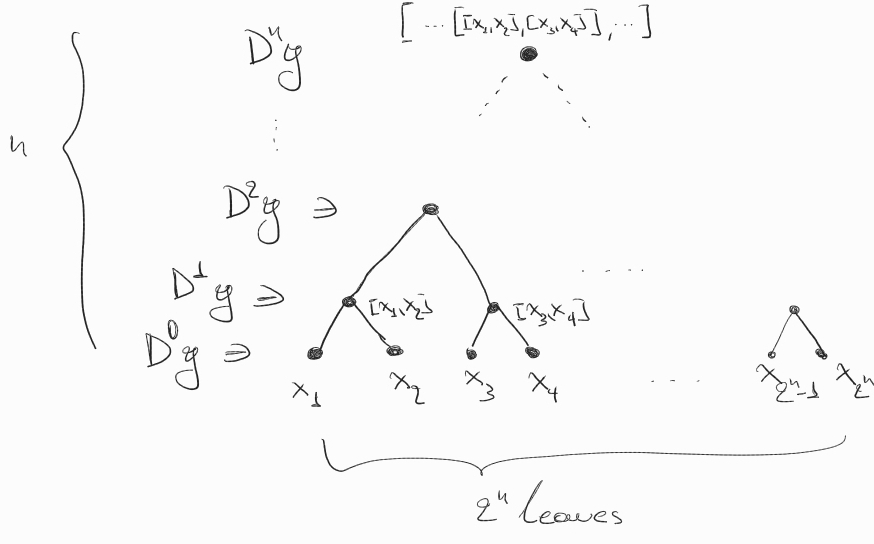
\includegraphics[width=\textwidth]{derived_series_tree.jpg}
        \caption{Illustration of derived series. Each node is the bracket of its children.}
        \label{fig:derived_series}
    \end{minipage}
    \hfill
    \begin{minipage}[b]{0.4\linewidth}
        \centering
        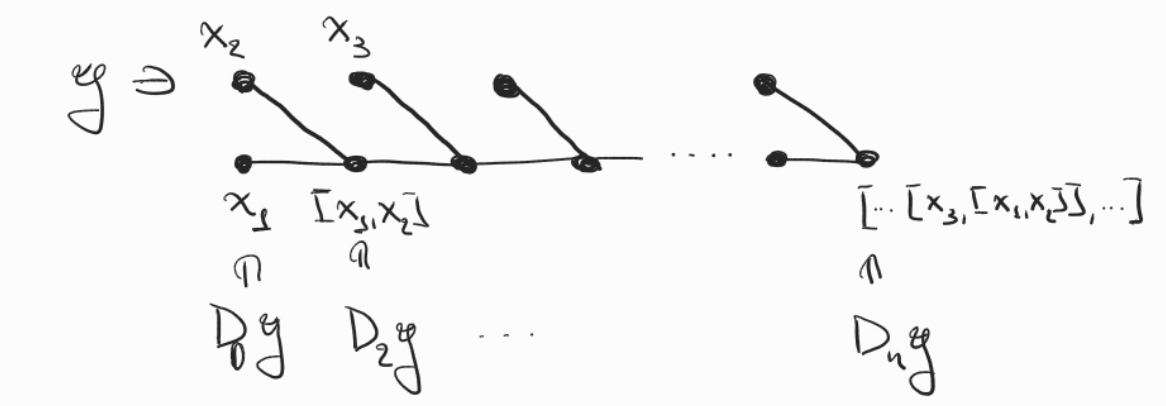
\includegraphics[width=\textwidth]{lower_central_series_graph.jpg}
        \caption{Illustration of lower central series. Each node is the bracket of its children.}
        \label{fig:lower_central_series}
    \end{minipage}
\end{figure}

Similar to the solvable algebras, we also have the notion of nilpotent algebras.
\begin{definition}
    Let $\mathfrak g$ be a Lie algebra. We define the lower central series of $\mathfrak g$ as the decreasing sequence of ideals, begining with $D_0 \mathfrak g = \mathfrak g$ and
    \[
    D_{i+1} \mathfrak g = [\mathfrak g, D_i \mathfrak g].
    \]
    The algebra is called nilpotent if one of the following conditions holds:
    \begin{enumerate}[label = (\roman*)]
        \item The lower central series terminates, i.e.\ there exists $n \in \mathbb N$ such that $D_n \mathfrak g = 0$.
        \item There exists a chain of ideals $\mathfrak a_0 = \mathfrak g \supseteq \mathfrak a_1 \supseteq \cdots \supseteq \mathfrak a_k = 0$ such that $[\mathfrak g, \mathfrak a_i] \subseteq \mathfrak a_{i+1}$.
        \item For large enough $n$, every commutator of the form $[x_1, [x_2, \ldots [x_{n-1}, x_n]\ldots]]$ ($n$ terms) is zero (see \cref{fig:lower_central_series}).
    \end{enumerate}
\end{definition}




An important example is $\mathfrak{gl}(n , \mathbb K)$.
Before we describe it, we make some preliminary remarks that will facilitate the computations.
We shall call $k$-diagonal of a matrix $a_{ij}$ the entries whose indices satisfy $i-j=k$, and denote with $A_k \subseteq \gl(n, \mathbb K)$ the additive group of matrices whose entries are zero below the $k$-diagonal (i.e.\ $a_{ij} \neq 0$ implies $i-j \leq k$).
Note then $A_k A_l \subseteq A_{k+l}$.

On the other hand, let $\mathcal F$ be a flag in a finite-dimensional vector space $V$, that is a chain of subspaces (without repetitions and without restriction on the dimensions of the subspaces):
\[
\mathcal F = \left\{ 0 \subsetneq V_1 \subsetneq V_2 \subsetneq \cdots \subsetneq V_n \right\}.
\]
Then we define:
\begin{align*}
    \mathfrak b(\mathcal F) &= \left\{ x \in \gl(V) : x V_i \subseteq V_i \text{ for all } i \right\}\\
    \mathfrak n(\mathcal F) &= \left\{ x \in \gl(V) : x V_i \subseteq V_{i-1} \text{ for all } i \right\}\\
    \mathfrak a_k(\mathcal F) &= \left\{ x \in \gl(V) : x V_i \subseteq V_{i - k} \right\}.
\end{align*}
Note that $\mathfrak b(\mathcal F) = \mathfrak a_0(\mathcal F)$ and $\mathfrak n(\mathcal F) = \mathfrak a_1(\mathcal F)$, while $\mathfrak a_{k} \mathfrak a_l, [\mathfrak a_k, \mathfrak a_l] \subseteq \mathfrak a_{k+l}$.
Using induction, this means that $D_i \mathfrak n(\mathcal F) \subseteq \mathfrak a_{i+1}$, 
so $\mathfrak n(\mathcal F)$ is nilpotent.
In particular, letting $\mathcal F = \mathcal F_0$ be the standard flag in $\mathbb K^n$, the algebras $\mathfrak a_k$ are the matrices that are zero below the $k$-th diagonal:
\[
\left\{ A : a_{ij} = 0 \text{ for } i - j > k
\right\}
\]
\begin{example}
    The commutator of $\mathfrak{gl}(n, \mathbb K)$ is given by
    \[
    [\gl(n, \mathbb K), \gl(n, \mathbb K)] = \ssl(n, \mathbb K).
    \]
    Let now $\mathfrak b \subseteq \gl(n, \mathbb K)$ be the subalgebra of upper triangular matrices and $\mathfrak n$ be the subalgebra of strictly upper triangular matrices.
    Then $\mathfrak b$ is solvable and $\mathfrak n$ is nilpotent.

    Noting that $\mathfrak b = \mathfrak b (\mathcal F_0), \mathfrak n = \mathfrak n(\mathcal F_0)$ for $\mathcal F_0$ being the standard flag in $\mathbb K^n$, we have seen above that $\mathfrak n$ is nilpotent.
    
    To see that $\mathfrak b$ is solvable, note that $D^1 \mathfrak b = [\mathfrak b, \mathfrak b] \subseteq \mathfrak n = \mathfrak a_i$ since the diagonal entries of $xy$ and $yx$ coincide.
    Inductively, this implies that $D^{i+1} \mathfrak b \subseteq \mathfrak a_{2^i}$.

    Note finally that $\mathfrak b $ is not nilpotent because $D_i \mathfrak b = \mathfrak n$.
    Indeed, we have seen that $D_1 \mathfrak b = [\mathfrak b, \mathfrak b] \subseteq \mathfrak n$.
    On the other hand, the relation 
    \[
    E_{ij} E_{kl} = \delta_{jk} E_{il}
    \]
    tells us that $E_{ij} = [E_{ii}, E_{ij}] \in D_2 \mathfrak b$, so $D_2 \mathfrak b = D_1 \mathfrak b = \mathfrak n$, so it follows by induction.
\end{example}

Finally, we have the following properties for solvable and nilpotent algebras.
\begin{proposition}
    \begin{enumerate}[label = (\roman*)]
        \item A real Lie algebra is solvable (resp.\ nilpotent) if and only if its complexification is.
        \item If $\mathfrak g$ is solvable (resp.\ nilpotent), then every subalgebra and quotient of $\mathfrak g$ is solvable (and resp.\ nilpotent).
        \item If $\mathfrak g$ is nilpotent, it is solvable.
        \item If $I \subseteq \mathfrak g$ is an ideal such that both $\mathfrak g, \mathfrak g/I$ are solvable, then $\mathfrak g$ is solvable.
    \end{enumerate}
\end{proposition}
\begin{proof}
For certain points, it is useful to note that if $I\subseteq \mathfrak g$ is an ideal, then $D^i \mathfrak (g/I) = (D^i \mathfrak g) + I$.
\end{proof}

\section{Lie algebra of vector fields}
For a manifold $M$, the space $\mathrm{Vect}(M)$ can be made into a Lie algebra by directly defining the bracket of two vector fields and showing that it is skew-symmetric and bilinear.
However, one can think of $\mathrm{Diff}(M)$ as similar to a Lie group (but not quite, since it is infinite-dimensional), whose Lie algebra is $\mathrm{Vect}(M)$.
\begin{definition}
    Let $M$ be a smooth manifold and $G$ be a Lie group.
    \begin{enumerate}[label = (\roman*)]
        \item A smooth map $\rho: G \to \mathrm{Diff}(M)$ is a map that arises from a smooth action of $G$ on $M$.
        \item The Lie algebra of $\mathrm{Diff}(M)$ is the space of vector fields $\mathrm{Vect}(M)$.
        \item The exponential map of $\mathrm{Diff}(M)$ is the flow (whenever well-defined) of a vector field: $\left(e^X\right)_m = \Phi^1_X(m)$.
        \item The differential of $\rho: G \to \mathrm{Diff}(M)$ is the map $\rho_*: \mathfrak g \to \mathrm{Vect}(M)$ given by
        \[
        \left(\rho_*(x)\right)_m = \left.\frac{\d}{\d t}\right|_{t=0} \rho\left(e^{tx}\right)(m).
        \]
        \item The commutator $[\xi, \eta]$ of two vector fields $\xi, \eta \in \mathrm{Vect}(M)$ is the unique vector field that satisfies
        \[
        \Phi^t_\xi \Phi^s_\eta \Phi^{-t}_\xi \Phi^{-s}_\eta = \Phi^{ts}_{[\xi, \eta]} + \cdots
        \]
        where the dots stand for terms of order 3 and higher in $s,t$.
    \end{enumerate}
\end{definition}

\begin{remark}
    To motivate why $\mathrm{Vect}(M) = \mathfrak{diff}(M)$, we note that $\mathfrak{diff}(M)$ should be given by the derivatives of the one-parameter subgroups of $\mathrm{Diff}(M)$.
    If $\phi^t \in \mathrm{Diff}(M)$ is a one-parameter subgroup of $M$, then its derivative defines a vector field $\partial_{t=0} \phi^t \in \mathrm{Vect}(M)$:
    \[
    \frac{\d}{\d t}\Big|_{t=0} \phi^t(m) \in T_m(M), \text{ for } m \in M.
    \]
    Similarly, to motivate the differential of $\rho: G \to \mathrm{Diff}(M)$, we note that $\rho$ maps one-parameter subgroups to one-parameter subgroups.
\end{remark}

\begin{proposition}[Proposition 3.23, \cite{kirillov2008introduction}]
    Let $M$ be a smooth manifold and $G$ be a Lie group acting smoothly on $M$.
    \begin{enumerate}[label = (\roman*)]
        \item The commutator of vector fields makes $\mathrm{Vect}(M)$ into a Lie algebra.
        \item The commutator can be also defined by the following formulas:
        \begin{align*}
            [\xi, \eta] &= \frac{\d}{\d t} (\Phi^t_\xi)_* \eta \\
            \partial_{[\xi, \eta]}f &= \partial_\eta \partial_\xi f - \partial_\xi \partial_\eta f\\
            \left[ f^i \partial_i, g^j \partial_j \right] &= \left( g^i \partial_i f^j - f^i \partial_i g^j \right) \partial_j
        \end{align*}
    \end{enumerate}
\end{proposition}
Note that the first expression from the second point of the above theorem should be read as
\[
[\xi, \eta]_p = \frac{\d}{\d t}\Big|_{t=0} d_{\Phi^{-t}_\xi(p)} \Phi^t_\xi (\eta_{\Phi^{-t}_\xi(p)})
\]
which allows us to interpret the Lie bracket of two vector fields as differentiation of the one along (the integral curves of) the other.

\begin{theorem}[Theorem 3.25, \cite{kirillov2008introduction}]
    The transformation $\rho_*: \mathfrak g \to \mathrm{Vect}(M)$ is a Lie algebra morphism.
\end{theorem}

\begin{example}
    \begin{enumerate}[label = (\roman*)]
        \item Considering the action of $G$ on itself by left-multiplication $L: G \to \mathrm{Diff}(G)$, the Lie algebra isomorphism
        \[
        L_*: \mathfrak g \leftrightarrow \{\text{right invariant vector fields on } \} G
        \]
        associates to $x \in \mathfrak g$ the right-invariant vector field $X$ such that $X_e = x$.
    \end{enumerate}
\end{example}

\section{Stabilizers and the center}
\begin{corollary}
    Let $f: G_1 \to G_2$ be a morphism of real or complex Lie groups.
    Then 
    \begin{enumerate}[label = (\roman*)]
        \item $\ker f $ is a closed Lie subgroup with Lie algebra $\ker f_*$.
        \item The map $G_1/\ker f \to \mathrm{Im} f$ is an immersion.
        \item When $\mathrm{Im}f$ is a submanifold, the map is a $G_1/\ker f \to \mathrm{Im}f$ diffeomorphism.
    \end{enumerate}
\end{corollary}

\begin{example}
    \begin{enumerate}[label = (\roman*)]
        \item 
        Let $V$ be a vector space over $\mathbb K$ with a bilinear form $B$.
        Then
        \[
        \mathrm{O}(V, B) = \left\{ g \in \GL(V) : B(gu, gv) = B(u,v) \text{ for all } u, v \in V \right\}
        \]
        is a closed Lie group with Lie algebra:
        \[
        \mathfrak{o}(V,B) = \left\{ g \in \mathfrak{gl}(V): B(xu, xv) = B(u,v) \text{ for all } u,v \in V\right\}.
        \]
    
        Indeed, define an action of $\GL(V)$ on the space $\mathcal F$ of bilinear forms on $V$ by $gF(u,v) = F(g^{-1}u, g^{-1}v)$.
        This defines a representation $\rho: \GL(V) \to \GL(\mathcal F)$ and $\mathrm{O}(V,B)$ is the stabilizer of $B$ under this action.
        The space $\mathcal F$ is a vector space, so $\mathrm{Vect}(\mathcal F)$ can be identifies with the space smooth maps from $\mathcal F$ to itself.
        Then for $x \in \mathfrak{gl}(V)$
        \begin{align*}
            \left(\rho_*(x)\right)_B(u,v) &= \left( \frac{\d}{\d t}\Big|_{t=0} \rho(e^{tx}) B\right)(u, v) = \left( \frac{\d}{\d t}\Big|_{t=0} B(e^{-tx}u, e^{-tx}v)\right)\\
            &= -B(u, xv) - B(xu, v).
        \end{align*}
    
        \item 
        Let $A$ be a finite-dimensional associative algebra over $\mathbb{K}$. Then the group of all automorphisms of $A$
        \[
        \text{Aut}(A) = \{g \in \text{GL}(A) \mid (g a) \cdot (g b) = g(a \cdot b) \text{ for all } a,b \in A\}
        \]
        is a Lie group with Lie algebra
        \[
        \text{Der}(A) = \{x \in \mathfrak{gl}(A) \mid (x.a)b + a(x.b) = x(ab) \text{ for all } a, b \in A\}
        \]
        (this Lie algebra is called the \textit{algebra of derivations of} $A$).
        
        Indeed, if we consider the space $W$ of all linear maps $A \otimes A \to A$ and define the action of $G$ by $(g f)(a \otimes b) = g f(g^{-1}a \otimes g^{-1}b)$ then $\text{Aut} A = G_\mu$, where $\mu : A \otimes A \to A$ is the multiplication. So $\text{Aut}(A)$ is a Lie group with Lie algebra $\text{Der}(A)$.
        \item 
        The same argument also shows that for a finite-dimensional Lie algebra $\mathfrak{g}$, the group
        \[
        \text{Aut}(\mathfrak{g}) = \{ g \in \text{GL}(\mathfrak{g}) \mid [ga, gb] = g[a, b] \text{ for all } a, b \in \mathfrak{g} \}
        \]
        is a Lie group with Lie algebra
        \[
        \text{Der}(\mathfrak{g}) = \{ x \in \mathfrak{gl}(\mathfrak{g}) \mid [x.a, b] + [a, x.b] = x.[a, b] \text{ for all } a, b \in \mathfrak{g} \}
        \]
        called the Lie algebra of derivations of $\mathfrak{g}$.
    \end{enumerate}
\end{example}


Finally, we can show that the center of $G$ is a closed Lie subgroup.


\begin{theorem}
Let $G$ be a connected Lie group. Then its center $Z(G)$ is a closed Lie subgroup with Lie algebra the ideal 
\[
\mathfrak{z}(\mathfrak{g}) = \{ x \in \mathfrak{g} \mid [x, y] = 0 \ \forall y \in \mathfrak{g} \}.
\]
\end{theorem}

The quotient group $G / Z(G)$ is usually called the \textit{adjoint group} associated with $G$ and denoted $\text{Ad}\, G$:
\[
\text{Ad}\, G = G / Z(G) = \text{Im}(\text{Ad}: G \rightarrow \text{GL}(\mathfrak{g})) \quad \text{(for connected } G).
\]
The corresponding Lie algebra is
\[
\text{ad}\, \mathfrak{g} = \mathfrak{g} / \mathfrak{z}(\mathfrak{g}) = \text{Im}(\text{ad}: \mathfrak{g} \rightarrow \mathfrak{gl}(\mathfrak{g})).
\]


\section{Campbell--Hausdorff formula}
So far, we have shown that the multiplication in a Lie group $G$ defines the
commutator in $g = T_1 G$. 
However, the definition of commutator only used the lowest non-trivial term of the group law in logarithmic coordinates. Thus, it might be expected that higher terms give more operations on g. However, it turns out that it is not so: the whole group law is completely determined by the lowest term, i.e.\ by the commutator, as follows from the Campbell--Hausdorff formula:
\begin{theorem}[Campbell--Hausdorff Formula]
    For small enough $x, y \in \mathfrak{g}$ one has
    \[
    \exp(x) \exp(y) = \exp(\mu(x, y))
    \]
    for some $\mathfrak{g}$-valued function $\mu(x, y)$ which is given by the following series convergent in some neighborhood of $(0, 0)$:
    \[
    \mu(x, y) = x + y + \sum_{n \geq 2} \mu_n(x, y), 
    \]
    where $\mu_n(x, y)$ is a Lie polynomial in $x, y$ of degree $n$, i.e. an expression consisting of commutators of $x, y$, their commutators, etc., of total degree $n$ in $x, y$. This expression is universal: it does not depend on the Lie algebra $\mathfrak{g}$ or on the choice of $x, y$.
    In particular, the group operation in a connected Lie group $G$ can be
    recovered from the commutator in $\mathfrak g$.
    \end{theorem}
    
    It is possible to write the expression for $\mu$ explicitly. 
    However, this is rarely useful, so we will only write the first few terms:
    \[
    \mu(x, y) = x + y + \frac{1}{2}[x, y] + \frac{1}{12} \left( [x, [x, y]] + [y, [y, x]] \right) + \cdots 
    \]
    

Although it follows from the Campbell--Hausdorff formula, the commutation criterion of the exponential can be also proven directly:
\begin{theorem}[Theorem 3.36, \cite{kirillov2008introduction}]
    Let $x, y \in \mathfrak g$.
    Then $e^x e^y = e^y e^x$ if and only if $[x,y]=0$.
    In that case $e^x e^y = e^y e^x = e^{x+y}$.
\end{theorem}
\begin{proof}
    The if direction follows from the definition of the commutator via Taylor series.
    For the other direction we follow the method suggested in Exercise 3.11 of \cite{kirillov2008introduction}:
    \[
    \Ad(e^x)y = e^{\ad x} y = \sum_{n\geq 0} \frac{(\ad x)^n}{n!} y = y
    \]
    But $C_g e^z = e^{\Ad_g z}$, so the above implies that $e^x e^y e^{-x} = C_{e^x}e^y = e^{\Ad(e^x)y} = e^y$.
\end{proof}

\section{Fundamental theorems of Lie theory}
Let us summarize the results we have so far about the relation between Lie
groups and Lie algebras.

\begin{enumerate}
    \item Every real or complex Lie group $G$ defines a Lie algebra $\mathfrak{g} = T_1 G$ (respectively, real or complex), with commutator defined by (3.2); we will write $\mathfrak{g} = \text{Lie}(G)$. Every morphism of Lie groups $\varphi : G_1 \to G_2$ defines a morphism of Lie algebras $\varphi_* : \mathfrak{g}_1 \to \mathfrak{g}_2$. For connected $G_1$, the map
    \[
    \text{Hom}(G_1, G_2) \to \text{Hom}(\mathfrak{g}_1, \mathfrak{g}_2)
    \]
    \[
    \varphi \mapsto \varphi_*
    \]
    is injective. (Here $\text{Hom}(\mathfrak{g}_1, \mathfrak{g}_2)$ is the set of Lie algebra morphisms.)
    \item As a special case of the previous, every Lie subgroup $H \subset G$ defines a Lie subalgebra $\mathfrak{h} \subset \mathfrak{g}$.
    \item The group law in a connected Lie group $G$ can be recovered from the commutator in $\mathfrak{g}$; however, we do not yet know whether we can also recover the topology of $G$ from $\mathfrak{g}$.
\end{enumerate}

However, this still leaves a number of questions.
\begin{question}
    Given a morphism of Lie algebras $\mathfrak{g}_1 \to \mathfrak{g}_2$, where $\mathfrak{g}_1 = \text{Lie}(G_1)$, $\mathfrak{g}_2 = \text{Lie}(G_2)$, can this morphism always be lifted to a morphism of the Lie groups?
\end{question}
\begin{question}
    Given a Lie subalgebra $\mathfrak{h} \subset \mathfrak{g} = \text{Lie}(G)$, does there always exist a corresponding Lie subgroup $H \subset G$?
\end{question}
\begin{question}
    Can every Lie algebra be obtained as a Lie algebra of a Lie group?
\end{question}

As the following example shows, in this form the answer to question 1 is negative.

\begin{example}
Let $G_1 = S^1 = \mathbb{R}/\mathbb{Z}, G_2 = \mathbb{R}$. Then the Lie algebras are $\mathfrak{g}_1 = \mathfrak{g}_2 = \mathbb{R}$ with zero commutator. Consider the identity map $\mathfrak{g}_1 \to \mathfrak{g}_2 : a \mapsto a$. Then the lift $\tilde f: \mathbb R \to \mathbb R$ of the corresponding morphism to the universal covering group (provided that the underlying morphism $f: \mathbb S^1 \to \mathbb R$ exists), should be given by $\tilde(\theta) = \theta + c$; on the other hand, it must also satisfy $\tilde f(\mathbb{Z}) = \{0\}$. Thus, this morphism of Lie algebras can not be lifted to a morphism of Lie groups.
\end{example}

In this example the difficulty arose because $G_1$ was not simply-connected. It turns out that this is the only difficulty: after taking care of this, the answers to all the questions posed above are positive. The following theorems give precise statements.

\begin{theorem}[First fundemental theorem of Lie theory]
For any real or complex Lie group $G$, there is a bijection between connected Lie subgroups $H \subset G$ and Lie subalgebras $\mathfrak{h} \subset \mathfrak{g}$, given by $H \mapsto \mathfrak{h} = \text{Lie}(H) = T_1 H$.
\end{theorem}

\begin{theorem}[Second fundemental theorem of Lie theory]
If $G_1, G_2$ are Lie groups (real or complex) and $G_1$ is connected and simply connected, then $\text{Hom}(G_1, G_2) = \text{Hom}(\mathfrak{g}_1, \mathfrak{g}_2)$, where $\mathfrak{g}_1, \mathfrak{g}_2$ are Lie algebras of $G_1, G_2$ respectively.
\end{theorem}

\begin{theorem}[Lie's third theorem]
Any finite-dimensional real or complex Lie algebra is isomorphic to a Lie algebra of a Lie group (respectively, real or complex).
\end{theorem}

These are the fundamental theorems of Lie theory and combining these with the previous results, we get the following important corollary.

\begin{corollary}[Le group and algebra equivalence]
    The categories of finite-dimensional Lie algebras and connected, simply-connected Lie groups are equivalent.
    In other words, for any real or complex finite-dimensional Lie algebra $\mathfrak{g}$, there is a unique (up to isomorphism) connected simply-connected Lie group $G$ (respectively, real or complex) with $\text{Lie}(G) = \mathfrak{g}$. Any other connected Lie group $G'$ with Lie algebra $\mathfrak{g}$ must be of the form $G/Z$ for some discrete central subgroup $Z \subset G$.
\end{corollary}

\section{Complex and real forms}
The operation of complexification, which is trivial at the level of Lie algebras,
is highly non-trivial at the level of Lie groups.
Real forms and their complexifications can be topologically quite different: for example, $\SU(n)$ is compact while $\SL(n, C)$ is not. On the other hand, it is natural to expect that their algebras share many algebraic properties, such as semisimplicity.
Thus we may use the properties of the complex Lie algebra to study the real Lie algebra, and vice versa, or use the properties of one real form to study another real form.
Thus, we may use, for example, use the compact group $\SU(n)$ to prove some results
about the non-compact group $\SL(n, C)$. Moreover, since $\mathfrak{sl}(n, \mathbb R)_{\mathbb C} = \mathfrak{sl}(n, \mathbb C)$,
this will also give us results about the non-compact real group $\SL(n, \mathbb R)$.

\begin{definition}
    \begin{enumerate}[label = (\roman*)]
        \item 
        The complexification $\mathfrak g_{\mathbb C}$ of a real Lie algebra $\mathfrak g$ is the complex Lie algebra
    \[
    \mathfrak g_{\mathbb C} \equaldef \mathfrak g \otimes_{\mathbb R} \mathbb C = \mathfrak g \oplus i \mathfrak g.
    \]
    We say that $\mathfrak g$ is a real form of $\mathfrak g_{\mathbb C}$.
    \item
    Let $G$ be a connected complex Lie group with Lie algebra $\mathfrak g$. 
    A closed real Lie subgroup $K \leq G$ is a real form of $G$ if its Lie algebra $\mathfrak k$ is a real form of $\mathfrak g$.
    \end{enumerate}
\end{definition}

In some cases, complexification is obvious, as in $\mathfrak g = sl(n, R)$.
Others however, are less obvious, as $\mathfrak g = \mathfrak u(n)$.
Finding a real form for a complex group is can be often direct:
\begin{proposition}
    Let $G$ be a connected simply-connected complex Lie group with Lie algebra $\mathfrak g$.
    Then every real form $\mathfrak k$ of $\mathfrak g$ is realised as the Lie algebra of a real form $K$ of $G$.
\end{proposition}
\begin{proof}
    Considering $\mathfrak g = \mathfrak k \oplus i \mathfrak k$, we define the real Lie algebra automorphism
    \[
    \theta: \mathfrak g \to \mathfrak g, \quad x + iy \mapsto x - iy.
    \]
    Since $G$ is connected and simply connected, the second fundamental theorem of Lie groups tells us that $\theta$ can be lifted to a Lie group automorphism $\Theta: G \to G$.
    Then $K = G^\Theta$ is a real form of $G$ with Lie algebra $\ker \theta = \mathfrak k$.
\end{proof}
Going in the opposite direction, from a real Lie group to a complex one, is
more subtle: there are real Lie groups that can not be obtained as real forms
of a complex Lie group (for example, it is known that the universal cover
of $\SL(2, \mathbb R)$ is not a real form of any complex Lie group). It is still possible
to define a complexification for any real Lie group G; however, in general the former does not admit the latter as a subgroup.


\chapter{Representations of Lie groups and Lie algebras}
In this chapter, we will discuss the representation theory of Lie groups and Lie
algebras. 
Unless specified otherwise, all Lie groups, algebras,
and representations are finite-dimensional, and all representations are complex.
Lie groups and Lie algebras can be either real or complex; unless specified
otherwise, all results are valid both for the real and complex case.

\section{Basic definitions}

\begin{definition}
    A representation of a Lie group \( G \) is a vector space \( V \) together with a morphism \( \rho : G \to \mathrm{GL}(V) \).
    
    A representation of a Lie algebra \( \mathfrak{g} \) is a vector space \( V \) together with a morphism \( \rho : \mathfrak{g} \to \mathfrak{gl}(V) \).
    
    A morphism between two representations \( V, W \) of the same group \( G \) is a linear map \( f : V \to W \) which commutes with the action of \( G \): \( f \rho(g) = \rho(g)f \). In a similar way, one defines a morphism of representations of a Lie algebra. The space of all \( G \)-morphisms (respectively, \( \mathfrak{g} \)-morphisms) between \( V \) and \( W \) will be denoted by \( \mathrm{Hom}_G(V, W) \) (respectively, \( \mathrm{Hom}_{\mathfrak{g}}(V, W) \)).
\end{definition}
    
\begin{remark}
Morphisms between representations are also frequently called \textit{intertwining operators} because they ``intertwine'' action of \( G \) in \( V \) and \( W \).
\end{remark}

The notion of a representation is completely parallel to the notion of module over an associative ring or algebra; the difference of terminology is due to historical reasons. In fact, it is also usual to use the word ``module'' rather than ``representation'' for Lie algebras: a module over Lie algebra \( \mathfrak{g} \) is the same as a representation of \( \mathfrak{g} \). We will use both terms interchangeably.

Note that in this definition we did not specify whether \( V \) and \( G \) are real or complex. Usually if \( G \) (respectively, \( \mathfrak{g} \)) is complex, then \( V \) should also be taken a complex vector space. However, it also makes sense to take complex \( V \) even if \( G \) is real: in this case we require that the morphism \( G \to \mathrm{GL}(V) \) be smooth, considering \( \mathrm{GL}(V) \) as \( 2n^2 \)-dimensional real manifold. Similarly, for real Lie algebras we can consider complex representations requiring that \( \rho : \mathfrak{g} \to \mathfrak{gl}(V) \) be \( \mathbb{R} \)-linear.
    
Of course, we could also restrict ourselves to consideration of real representations of real groups. However, it turns out that the introduction of complex representations significantly simplifies the theory even for real groups and algebras. Thus, from now on, all representations will be complex unless specified otherwise.
    
\begin{example}
    For a Lie group $G$ or a Lie algebra $\mathfrak g$ we always have the following two representations:
    \begin{enumerate}[label = (\roman*)]
        \item Trivial representation: $V = \mathbb C, \rho(g) = \id$ for all $g \in G$ (respectively $\rho(x) = 0$ for all $x \in \mathfrak g$). 
        \item Adjoint representation: $V = \mathfrak g, \rho(g) = \Ad_g$ for all $g \in G$ (respectively $\rho(x) = \ad_x$ for all $x \in \mathfrak g$). 
        \item Coadjoint representation: $V = \mathfrak g^*, \rho(x) = \ad_x^* $ for all $x \in \mathfrak g$.
    \end{enumerate}
\end{example}

The first important result about representations of Lie groups and Lie algebras is the following theorem.
It tells us that from a representation (or a morphism of representations) of a Lie group we can obtain a representation (or a morphism of representations) of its Lie algebra, and that when $G$ is connected, simply connected, then representing $G$ and representing its Lie algebra is equivalent.
\begin{theorem}
Let \( G \) be a Lie group (real or complex) with Lie algebra \( \mathfrak{g} \).
\begin{enumerate}
    \item Every representation \( \rho : G \to \mathrm{GL}(V) \) defines a representation \( \rho_* : \mathfrak{g} \to \mathfrak{gl}(V) \), and every morphism of representations of \( G \) is automatically a morphism of representations of \( \mathfrak{g} \).
    \item If \( G \) is connected, simply-connected, then \( \rho \mapsto \rho_* \) gives an equivalence of categories of representations of \( G \) and representations of \( \mathfrak{g} \). In particular, every representation of \( \mathfrak{g} \) can be uniquely lifted to a representation of \( G \), and \( \mathrm{Hom}_G(V, W) = \mathrm{Hom}_{\mathfrak{g}}(V, W) \).
\end{enumerate}
\end{theorem}
This is an important result, as Lie algebras are, after all, finite dimensional vector spaces, so they are easier to deal with.
\begin{example}
    A representation of \( \mathrm{SU}(2) \) is the same as a representation of \( \mathfrak{su}(2) \), i.e. a vector space with three endomorphisms \( X, Y, Z \), satisfying commutation relations \( XY - YX = Z, YZ - ZY = X, ZX - XZ = Y \).
\end{example}
\begin{remark}
    This theorem can also be used to describe representations of a group which is connected but not simply-connected, in the sense that representations of $G$ are the same as representations of its universal cover that are trivial over the fundamentla group of $G$.
    More concretely, any such group $G$ can be written as \( G = \tilde{G}/Z \) for some simply-connected group \( \tilde{G} \) and a discrete central subgroup \( Z \subset G \). Thus, representations of \( G \) are the same as representations of \( \tilde{G} \) satisfying \( \rho(Z) = \mathrm{id} \). An important example of this is when \( G = \mathrm{SO}(3, \mathbb{R}) \), \( \tilde{G} = \mathrm{SU}(2) \).
\end{remark}

\begin{lemma}
    Let $\mathfrak g $ be a real Lie algebra and $\mathfrak g_{\mathbb C}$ its complexification.
    Then the categories of complex representations of $mathfrak g$ and $\mathfrak g_{\mathbb C}$ are equivalent.
\end{lemma}
The next example shows that we can reduce the problem of study of representations of a non-compact Lie group $\SL(2, \mathbb C)$ to 
\begin{example}
    The categories of finite-dimensional representations of $\SL(2, \mathbb C)$,
$\SU(2)$, $\mathfrak{sl}(2, \mathbb C)$ and $\su(2)$ are all equivalent. Indeed,
$\mathfrak{sl}(2, C) = (\su(2))_{\mathbb C}$ , so categories of their finite-dimensional representations are equivalent; since the groups $\SU(2), \SL(2, C)$ are simply-connected, they
have the same representations as the corresponding Lie algebras.
\end{example}

\section{Operations on representations}
\subsection{Subrepresentations and quotients}

\begin{definition}
    Let $V$ be a representation of $G$ (respectively $\mathfrak g$). 
    A subrepresentation is a vector subspace $W \subseteq V$ stable under the action:
    $\rho(g)W \subseteq W$ for all $g \in G$ (respectively, $\rho(x)W \subseteq W$ for all $x \in \mathfrak g$).
\end{definition}

When $W \subseteq V$ is a subrepresentation, then one can obtain the factor representation or quotient representation $V/W$ given by
\[
\rho_{V/W}(g) = \rho_V(g) + W.
\]


\subsection{Direct sum and tensor product}
\begin{lemma}\label{lem:direct_sum_tensor_product}
    Let $V , W$ be representations of $G$ (respectively, $\mathfrak g$). 
    Then there is a canonical structure of a representation on $V^*, V \oplus W, V \otimes W$.
\end{lemma}
\begin{proof}
    It is given by
    \begin{align*}
        \rho(g)(v + w) &= \rho(g)(v) + \rho(g)(w) \text{ on } V \oplus W \text{ for } G,\\
        \rho(x)(v + w) &= \rho(x)(v) + \rho(x)(w) \text{ on } V \oplus W \text{ for } \mathfrak g,\\
        \rho(g)(v \otimes w) &= \rho(g)(v) \otimes \rho(g)(w) \text{ on } V \otimes W \text{ for } G,\\
        \rho(x)(v \otimes w) &= \rho(x)(v) \otimes w + v \otimes \rho(x)(w) \text{ on } V \otimes W \text{ for } \mathfrak g,\\
        \rho_{V^*}(g) &= \rho(g^{-1})^t \text{ on } V^* \text{ for } G,\\
        \rho_{V^*}(x) &= -\rho(x)^t \text{ on } V^* \text{ for } \mathfrak g,
    \end{align*}
    where we denote with $A^t$ the adjoint opearor $A^t:V^* \to V^*$ for $A: V \to V$.
\end{proof}
For example, the coadjoint representation is obtained by dualizing the adjoint representation of $\mathfrak g$.

Before giving the next series of examples, recall that for any finite dimensional vector spaces $V, W$, we have the following cannonical isomorphism:
\begin{align*}
    V^* \otimes W &\simeq \hom(V, W)\\
    f \otimes w &\mapsto \left( u \mapsto f(u)w \right)\\
    e^i \otimes (Ae_i) &\mapsfrom A
\end{align*}
where $e_1, \ldots, e_n$ are any basis of $V$ and $e_1, \cdots, e^n$ are its dual basis for $V^*$.

\begin{example}
    \begin{enumerate}[label = (\roman*)]
        \item Coadjoint representation on $\mathfrak g^*$: Dualizing the adjoint representation of $\mathfrak g$ we obtain the coadjoint representation given by $\rho(x) = ad_x^*$
        \item $\hom(V,W)$: Given two representations $V, W$ of $G$, the space of linear maps $\hom(V,W)$ is a representation by:
        \begin{align*}
            \rho(g)_{\hom(V,W)}(A) &= \rho_V(g)A\rho_W(g^{-1}) \text{ for } g \in G,\\
            \rho(x)_{\hom(V,W)}(A) &= \rho_V(x)A - A\rho_W(x) \text{ for } x \in \mathfrak g.
        \end{align*}
        This is obtained by dualizing and tensoring as in the lemma above, i.e.\ the diagram below is commutative\\
        \begin{center}
            \begin{tikzcd}
                V \otimes W^* \arrow[r, "\simeq"] \arrow[d, "\rho(g)"] & \hom(V,W) \arrow[d, "\rho(g)"] \\
                V \otimes W^* \arrow[r, "\simeq"] & \hom(V,W)
            \end{tikzcd}    
        \end{center}
        \item Bilinear forms: Given a representation $V$, the space of bilinear forms on $V$ becomes a representation when we consider it as a subspace of $V^* \otimes V^*$. It is given by:
        \begin{align*}
            g B(u, v) &= B(g^{-1}u, g^{-1}v), \text{ for } g \in G\\
            x B(u, v) &= -B(x u, v) - B(u, x v), \text{ for } x \in \mathfrak g.    
        \end{align*}
    \end{enumerate}
\end{example}

\subsection{Invariants}
\begin{definition}
    Let $V$ be a representation of a Lie group $G$. A vector $v \in V$ is
    called invariant if $\rho(g)v = v$ for all $g \in G$. The subspace of invariant vectors
    in $V$ is denoted by $V^G$.
    Similarly, let $V$ be a representation of a Lie algebra $\mathfrak g$. A vector $v \in V$ is
    called invariant if $\rho(x)v = 0$ for all $x \in g$. The subspace of invariant vectors
    in $V$ is denoted by $V^{\mathfrak g}$ .
\end{definition}

\begin{remark}
    When $G$ is connected, and $V$ is a representation of $G$, then
    \[
    V^G = V^{\mathfrak g}
    \]
\end{remark}

\begin{example}
    \begin{enumerate}[label = (\roman*)]
        \item $\hom(V, W)$: Considering $\hom(V,W)$ as the representation arising from two representations $V, W$, we have $\hom(V, W)^G = \hom_G(V, W)$.
        \item Bilinear forms: We have $B \in V^G$ if and only if the linear map $V \to V^*$, given by $v \to B(v, -)$, is a representations morphism.
    \end{enumerate}
\end{example}

\section{Irreducible representations}
One of the main problems of the representation theory is the problem of classi-
fication of all representations of a Lie group or a Lie algebra. In this generality,
it is an extremely difficult problem and for a general Lie group, no satisfactory
answer is known. We will later show that for some special classes of Lie groups
(namely compact Lie groups and semisimple Lie groups, to be defined later)
this problem does have a good answer.
The most natural approach to this problem is to start by studying the sim-
plest possible representations, which would serve as building blocks for more
complicated representations.

\begin{definition}
    \begin{enumerate}[label = (\roman*)]
        \item A non-zero representation V of $G$ or $\mathfrak g$ is called irreducible
        or simple if it has no subrepresentations other than $0$ and $V$ . 
        Otherwise $V$ is called reducible.
        \item $V$ is a completely completely reducible or semisimple representation if it is isomorphic to a direct sum of irreducible representations:
        $V = \oplus_i V_i$, with $V_i$ irreducible.
        \item If $V$ is completely reducible, one usually groups together isomorphic summands writing $V = \oplus_i n_i V_i$, where $V_i$ are pair-wise non-isomorphic irreducible
        representations and the numbers $n_i$ are called multiplicities.
    \end{enumerate}
\end{definition}
\begin{remark}
    Sometimes, it will be useful to consider the isomorphic expressions:
    \[
    n V \simeq \oplus_1^n V \simeq \mathbb C^n \otimes V
    \]
    where the latter isomorphism is given by the map $(v_1, \cdots, v_n) \mapsto e_1 \otimes v_1 + \cdots  e_n \otimes v_n $ and in the other direction by the map $z \otimes v \mapsfrom (z_1v, \cdots, z_n v)$.
\end{remark}

Thus, more modest goals of the representation theory would be answering
the following questions:
\begin{enumerate}[label = (\roman*)]
    \item For a given Lie group $G$, classify all irreducible representations of G.
    \item For a given representation $V$ of a Lie group G, given that it is completely reducible, find explicitly the decomposition of $V$ into direct sum of irreducibles.
    \item For which Lie groups $G$ all representations are completely reducible?
\end{enumerate}

\begin{example}[Irreducible representations]
    \begin{enumerate}[label = (\roman*)]
        \item $\mathbb C^n$: It is irreducible as a representation of $\SL(n, \mathbb C), \GL(n, \mathbb C)$.
    \end{enumerate}
\end{example}

\begin{example}[Reducible representations]
    \begin{enumerate}[label = (\roman*)]
        \item $\mathbb R$: It is reducible but not completely reducible as a representation of $\mathbb R$ (either seen as a group, or a Lie algebra).
        \item $\mathbb C^n \otimes \mathbb C^n$: It is completely reducible as a representation of $\GL(n, \mathbb C)$, since $\mathbb C^n \otimes \mathbb C^n = S^2 \mathbb C^n \oplus \Lambda^2 \mathbb C^n$, where $S^2 \mathbb C^n$ is the symmetric tensor product and $\Lambda^2 \mathbb C^n$ is the antisymmetric tensor product.
        \item Unitary representations are completely irreducible (see \cref{thm:unitary_implies_completeley_reducible}).
        This includes in particular representations of compact groups (see \cref{thm:compact_implies_unitary}).
        \item $\mathfrak{sl}(2, \mathbb C)$: Putting aside that we can classify all its finite-dimensional representations: any representation of $V$ is completely reducible, and any irreducible representation is isomorphic to a highest weight representation (see \cref{thm:irreducible_representations_of_sl2}).
    \end{enumerate}
\end{example}
\begin{proof}
    \begin{enumerate}[label = (\roman*)]
        \item\label{ex:R_not_completely_irreducible} 
        Looking at the Lie algebra $\mathfrak g = \mathbb R$, representations on $V$ are linear maps $\rho_*: \mathbb R \to \mathfrak{gl}(V)$ who will have the form $t \mapsto t A$, where $A = \rho_*(1)$. 
        Hence representations of $G = \mathbb R$ are the Lie group morphisms $\mathbb R \to \GL(d, \mathbb C)$ that have the form $t \mapsto e^{tA}$, where $A = \rho_*(1) \in \mathfrak{gl}(\mathbb C, d)$.
        If $v \in V$ is an eigenvector of $A$, then $\mathbb Cv$ is a subrepresentation in $V$, so the only irreducible representations of $\mathbb R$ are one-dimensional.
        In fact, $t \mapsto e^{tA}$ is completely irreducible if and only if $A$ is diagonalizable.
        Hence, the irreducible ones are given as the linear maps $\rho_*: \mathbb R \to \mathfrak{gl}(V) \simeq \mathbb C, t \mapsto t \lambda$, for some $\lambda = \lambda_{\rho_*} \in \mathbb C$, and the corresponding representation of $G$ is given by $\rho: \mathbb R \to \GL(V) \simeq \mathbb C^{\times}, t \mapsto e^{t \lambda}$.
    \end{enumerate}
\end{proof}

One tool which can be used in decomposing representations into direct sum
is the use of central elements.
\begin{lemma}
    Let $V$ be a representation of a Lie group $G$ (or a Lie algebra $\mathfrak g$ respectively).
    \begin{enumerate}[label = (\roman*)]
        \item Let $A \in \hom_G(V, V)$ be a diagonalizable interwining operator. 
        Then each eigenspace $V_\lambda$ of $A$ is an invariant subspace and we have the decomposition $V = \oplus V_\lambda$ into subrepresentations.
        \item If $Z \in Z(G)$ is a central element such that $\rho(Z)$ is diagonalizable, then as a representation of $G$, $V$ decomposes into a direct sum of eigenspaces of $\rho(Z)$: $V = \oplus V_\lambda$. 
    \end{enumerate} 
\end{lemma}

Of course, there is no guarantee that $V_\lambda$ will be an irreducible representation;
moreover, in many cases the Lie groups we consider have no central elements
at all.

\section{Intertwining operators and Schur’s lemma}
In this section we consider the following questions:
\begin{question}\label{q:invariance_eigenvalues}
How can $G$-invariance of an operator $A \in \mathfrak{gl}(V)$ helps computing eigenvalues and eigenspaces?
\end{question}

\begin{question}\label{q:centre_classical_lie_groups}
    What is an easy way to compute the centre of classical Lie groups?
\end{question} 

The following Lemma can be seen as a way to answer these questions:
\begin{lemma}[Schur's lemma]
    \begin{enumerate}[label = (\roman*)]
        \item Let $V$ be an irreducible representation of a Lie group $G$ (similar result holds for representations of a Lie algebra $\mathfrak g$.).
        Then the space of intertwining operators is one-dimensional:
        \[
        \hom_G(V, V) = \mathbb C \id.
        \]
        \item Let $V, W$ be irreducible representations of a Lie group $G$ which are not isomorphic.
        Then $\hom_G(V, W) = 0$.
    \end{enumerate}
\end{lemma}

\begin{example}[Answer to \cref{q:centre_classical_lie_groups}]
Consider the group \( \mathrm{GL}(n, \mathbb{C}) \). Since \( \mathbb{C}^n \) is irreducible as a representation of \( \mathrm{GL}(n, \mathbb{C}) \), every operator commuting with \( \mathrm{GL}(n, \mathbb{C}) \) must be scalar. Thus, the center \( Z(\mathrm{GL}(n, \mathbb{C})) = \{ \lambda \cdot \mathrm{id}, \lambda \in \mathbb{C}^\times \} \); similarly, the center of the Lie algebra is \( Z(\mathfrak{gl}(n, \mathbb{C})) = \{ \lambda \cdot \mathrm{id}, \lambda \in \mathbb{C} \} \).

Since \( \mathbb{C}^n \) is also irreducible as a representation of \( \mathrm{SL}(n, \mathbb{C}) \), \( \mathrm{U}(n) \), \( \mathrm{SU}(n) \), \( \mathrm{SO}(n, \mathbb{C}) \), a similar argument can be used to compute the center of each of these groups. The answer is
\[
\begin{array}{ll}
Z(\mathrm{SL}(n, \mathbb{C})) = Z(\mathrm{SU}(n)) = \{\lambda \cdot \mathrm{id}, \, \lambda^n = 1 \} & \mathfrak{z}(\mathrm{U}(n)) = \{ \lambda \cdot \mathrm{id}, \, |\lambda| = 1 \} \\
Z(\mathfrak{sl}(n, \mathbb{C})) = Z(\mathfrak{su}(n)) = 0 & \mathfrak{z}(\mathfrak{u}(n)) = \{ \lambda \cdot \mathrm{id}, \, \lambda \in i\mathbb{R} \} \\
Z(\mathrm{SO}(n, \mathbb{C})) = Z(\mathrm{SO}(n, \mathbb{R})) = \{\pm 1\} & \mathfrak{z}(\mathfrak{so}(n, \mathbb{C})) = \mathfrak{z}(\mathfrak{so}(n, \mathbb{R})) = 0.
\end{array}
\]
\end{example}

To answer \cref{q:invariance_eigenvalues}, we can use the following corollary of Schur's lemma:
\begin{corollary}
Let \( V \) be a completely reducible representation of Lie group \( G \) (respectively, Lie algebra \( \mathfrak{g} \)). Then
\begin{enumerate}
    \item If \( V = \bigoplus V_i \), \( V_i \) irreducible, pairwise non-isomorphic, then any intertwining operator \( \Phi : V \to V \) is of the form \( \Phi = \bigoplus \lambda_i \mathrm{id}_{V_i} \).
    \item If \( V = \bigoplus n_i V_i = \bigoplus n_i \mathbb{C}^{n_i} \otimes V_i \), \( V_i \) irreducible, pairwise non-isomorphic, then any intertwining operator \( \Phi : V \to V \) is of the form \( \Phi = \bigoplus (A_i \otimes \mathrm{id}_{V_i}) \), where \( A_i \in \mathrm{End}(\mathbb{C}^{n_i}) \).
\end{enumerate}
\end{corollary}

\begin{proof}
For part (1), notice that any operator \( V \to V \) can be written in a block form: \( \Phi = \bigoplus \Phi_{ij}, \Phi_{ij} : V_i \to V_j \). By Schur's lemma, \( \Phi_{ij} = 0 \) for \( i \neq j \) and \( \Phi_{ii} = \lambda_i \mathrm{id}_{V_i} \). Part (2) is proved similarly.
\end{proof}

This result shows that indeed, if we can decompose a representation \( V \) into irreducible ones, this will give us a very effective tool for analyzing intertwining operators. For example, if \( V = \bigoplus V_i, V_i \neq V_j \), then \( \Phi = \bigoplus \lambda_i \mathrm{id}_{V_i} \), so one can find \( \lambda_i \) by computing \( \Phi(v) \) for just one vector in \( V_i \). It also shows that each eigenvalue \( \lambda_i \) will appear with multiplicity equal to \( \dim V_i \). This is exactly what we did in the baby example above, only now \( V_i \) was one-dimensional, where we had \( G = \mathbb{Z}_n \).

We also have the following corrolary on commutative groups and algebras.
\begin{proposition}
    If $G$ is a commutative group, then any irreducible complex
representation of $G$ is one-dimensional. Similarly, if $\mathfrak g$ is a commutative Lie algebra, then any irreducible complex representation of $\mathfrak g$ is one-dimensional.
\end{proposition}
Now we are ready to give a classification of irreducible representations of $\mathbb R$ and $\mathbb S^1$
\begin{example}\label{ex:irreducible_representations_of_R}
    Let $G = \mathbb R$.
    Then the only irreducible representations of $G$ are one-dimensional (which follows either from the proposition above, or from \cref{ex:irreducible_representations_of_R}), and are given by $t \mapsto e^{\lambda t} $ for some $\lambda \in \mathbb C$.
    Similarly, the only irreducible representations of $\mathbb S^1 = \mathbb R/ \mathbb Z$ are one-dimensional complex spaces $V_k$ for $k \in \mathbb Z$, and are given by $t \mapsto e^{2\pi i k t}$.
\end{example}

\section{Complete irreducibility of unitary representations, representations on finite groups}

\begin{definition}
    A complex representation $V$ of a real group $G$ is unitary if there exists a $G$-invariant inner-product (i.e.\ positive Hermitian form) on $V$: $\rho(G) \subseteq U(V)$.
    Similarly, a representation $V$ of a Lie algebra $\mathfrak g$ is unitary if there exists a $\mathfrak g$-invariant inner-product on $V$: $\rho(\mathfrak g) \subseteq \mathfrak u(V)$, or equivalently $(\rho(x)v, w) + (v, \rho(x)w) = 0$ for all $x \in \mathfrak g, v, w \in V$.
\end{definition}

\begin{theorem}\label{thm:unitary_implies_completeley_reducible}
    Unitary representations are completely reducible.
\end{theorem}

\begin{example}[Unitary representations]
    \begin{enumerate}[label = (\roman*)]
        \item If $G$ acts by permutations on a finite set $S$, then the representation $\rho(g)f \equaldef f \circ g^{-1}$ on the space $F(S)$ of complex functions over $S$ is unitary.
        \item Representations of finite groups.
        \item Representations of compact groups (see \cref{thm:compact_implies_unitary}), e.g.\ finite groups, $\SU(n)$, $\SO(n)$, $\mathrm{U}(n)$, $\mathrm{SO}(n)$.
    \end{enumerate}
\end{example}

\section{Haar measure on compact Lie groups}
Since the proof that finite group representations are unitary is based on the existence of a right-invariant integral on the group, it is natural to ask whether a similar result holds for a broader class of Lie groups.

\begin{definition}
    A right Haar measure on a Lie group $G$ is a measure $\mu$ on $G$ that is invariant under the right action of $G$ on itself: $R_g^* \mu = \mu$.
    Equivalently $\int_G f(g) d\mu(g) = \int_G f(gh) d\mu(g)$ for all $h \in G$ and integrable functions $f$ on $G$.
\end{definition}

\begin{theorem}
    Let $G$ be a real Lie group.
    \begin{enumerate}
        \item Then $G$ is orientable and admits an orientation that is invariant under the right action of $G$ on itself.
        \item If $G$ is compact, then for a fixed choice of right-invariant orientation on $G$, there exists a unique right-invariant top degree non-vanishing differential form $\omega$ such that $\int_G \omega = 1$.
        This form is left-invariant and left-invariant  and invariant up to a sign under $i: g 
    \mapsto g^{-1}, i^*\omega = (-1)^{\dim G} \omega$.
    \end{enumerate}
\end{theorem}

\begin{theorem}
    Let $G$ be a compact Lie group.
    Then $G$ admits a right Haar measure, which is a Borel measure, and invariant under the right and left actions of $G$ on itself, and under inversion $i: g \mapsto g^{-1}$.
\end{theorem}

\begin{example}
    The Haar measure for $G= S^1 = \mathbb R/ \mathbb Z$ is the Lebesgue measure $\d x$ on $[0, 1]$.
\end{example}

\begin{theorem}\label{thm:compact_implies_unitary}
    Any finite-dimensional representation of a compact Lie group is unitary and thus completely reducible.
\end{theorem}

\section{Orthogonality of characters and Peter--Weyl theorem}
Throughout this section, we will assume that $G$ is a compact real Lie group with Haar measure $\d g$.
In the previous section, we saw that it is completely reducible, but we have no way of knowing what the factors of $G$ are, or what the multiplicities are.
This is what we will try to discuss in this section.

When $V$ is a representation of $G$ and $v_i$ a basis for $V$, we can consider the matrix corresponding to $\rho(g) \in \GL(V)$ in this basis, and denote with $\rho_{ij}$ its coefficients.
In this way we obtain scalar-valued functions $\rho_{ij}(g)$ on $G$.

We will make use of the following inner product on functions over $G$:
\begin{equation}\label{eq:inner_product}
    (f, g) = \int_G f(g) \overline{g(g)} \d g.
\end{equation}

The next theorem tells us that irreducible representations of a compact Lie group $G$ can give us an orthogonal set of functions on $G$.
\begin{theorem}
    Let $G$ be a compact real Lie group with Haar measure $\d g$.
    \begin{enumerate}[label = (\roman*)]
        \item Let $V, W$ be non-isomorphic irreducible representations of $G$ with basis $v_i, w_a$.
        Then the corresponding matrix coefficients are orthogonal:
        \[
        \left( \rho^V_{ij}, \rho^W_{ab} \right) = 0
        \]
        for all $i,j,a,b$, where the inner-product is defined as in \cref{eq:inner_product}.
        \item Let $V$ be an irreducible representation of $G$, and $v_i$ be an orthonormal basis with respect to a $G$-invariant inner product.
        Then the matrix coefficients $\rho_{ij}(g)$ are orthogonal:
        \[
        \left(\rho_{ij}, \rho_{kl} \right) = \frac{ \delta_{ik} \delta_{jl} }{\dim V}.
        \]
    \end{enumerate}
\end{theorem}

It is evident though that the set of matrix coefficients does depend on the choice of basis for the vector spaces.
For this reason, one considers a linear combination of coefficients that is basis-independent.

\begin{definition}
    A character of a representation $V$ of a real Lie group $G$ is the scalar function on the group defined by
    \[
    \chi_V(g) = \tr_V \rho(g) = \sum_i \rho_{ii}(g),
    \]
    where $\rho_{ij}(g)$ are the matrix coefficients of $\rho(g)$ in some basis of $V$.
\end{definition}
We have the following properties:
\begin{proposition}
    Let $V$ be a representation of a real Lie group $G$.
    \begin{enumerate}[label = (\roman*)]
        \item If $V = \mathbb C$ is the trivial representation, then $\chi_V(g) = 1$.
        \item $\chi_{V \oplus W} = \chi_V + \chi_W$.
        \item $\chi_{V \otimes W} = \chi_V \chi_W$.
        \item Characters are conjugation invariant: $\chi_V(hgh^{-1}) = \chi_V(g)$.
        \item If $G$ is compact, then $\chi_{V^*} = \overline{\chi_V}$.
    \end{enumerate}
\end{proposition}

The following theorem which follows from the orthogonality of matrix coefficients, tells us that characters of irreducible representations of a compact Lie group form an orthogonal family of functions on $G$.
\begin{theorem}
    Let $G$ be a compact real Lie group with Haar measure $\d g$.
    \begin{enumerate}[label = (\roman*)]
        \item Characters of non-isomorphic irreducible representations of $G$ are orthogonal:
        \[
        \left( \chi_V, \chi_W \right) = 0
        \]
        for all non-isomorphic irreducible representations $V, W$.
        \item For any representation $V$ of $G$ we have 
        \[
            \left( \chi_V, \chi_V \right) = 1 \text{ if and only if } V \text{ is irreducible}.
        \]
        \item The set $\left\{ \chi_V : V \in \hat G \right\}$ is an orthonormal family of functions of $G$, where $\hat G$ is the set of isomorphism classes of irreducible representations of $G$.
        \item For any representation $V$ of $G$ we can compute its multiplicities via:
        \[
        n_i = \left( \chi_V, \chi_{V_i} \right),
        \]
        where $V = \oplus_i n_i V_i$, and $V_i$ are pair-wise non-isomorphic irreducible representations.
    \end{enumerate}
\end{theorem}
Note that the last part of the theorem implies in particular that the factors and the multiplicities of a completely reducible representation of a compact Lie group can be computed from its character and are unique.

    
Returning to the matrix coefficients of representations, one might ask whether it is possible to give a formulation of their orthogonality in a way that does not require a choice of basis. The answer is “yes”. Indeed, let \( v \in V \), \( v^* \in V^* \). Then we can define a function on the group \( \rho_{v^*, v}(g) \) by
\[
\rho_{v^*, v}(g) = \langle v^*, \rho(g)v \rangle,
\]
and this correspondence extends to a mapping $ V^* \otimes V \rightarrow C^\infty(G, \mathbb{C})$
This is a generalization of a matrix coefficient: if \( v = v_j, v^* = v_j^* \), we recover matrix coefficient \( \rho_{ij}(g) \).

The space \( V^* \otimes V \) has additional structure. First, we have two commuting actions of \( G \) on it, given by action on the first factor and on the second one; in other words, \( V^* \otimes V \) is a \( G \)-bimodule. In addition, if \( V \) is unitary, then the inner product defines an inner product on \( V^* \) (the simplest way to define it is to say that if \( v_i \) is an orthonormal basis in \( V \), then the dual basis \( v_i^* \) is an orthonormal basis in \( V^* \)). Define an inner product on \( V^* \otimes V \) by
\begin{equation}\label{eq:inner_product_tensors}
    \langle v_1^* \otimes w_1, v_2^* \otimes w_2 \rangle = \frac{1}{\dim V} \langle v_1^*, v_2^* \rangle \langle w_1, w_2 \rangle.
\end{equation}

\begin{theorem}[Peter-Weyl theorem]
Let \( \hat{G} \) be the set of isomorphism classes of irreducible representations of \( G \). Define the map
\begin{align*}
    m : \bigoplus_{V_i \in \hat{G}} V_i^* \otimes V_i &\rightarrow C^\infty(G, \mathbb{C}), 
\text{ by}\\
    v^* \otimes v &\mapsto \langle v^*, \rho(\cdot)v \rangle.  
\end{align*}
Then
\begin{enumerate}[label = (\roman*)]
    \item $m$ is an isomorphism of \( G \)-bimodules, i.e.\ it is a linear isomorphism that commutes with the actions of \( G \) on the domain and the codomain:
    \begin{align*}
        m((gv^*) \otimes v) &= L_g(m(v^* \otimes v)),\\
        m(v^* \otimes (gv)) &= R_g(m(v^* \otimes v)),
    \end{align*}
    where $R_g, L_g$ are the right and left actions of $G$ on $C^\infty(G, \mathbb{C})$ given by $(R_g f)(x) = f(xg)$ and $(L_g f)(x) = f(g^{-1}x)$.
    \item The map $m$ extends to a Hilber spaces isomorphism:
    \[
    \hat{\bigoplus}_{V_i \in \hat{G}} V_i^* \otimes V_i \overset{\simeq}{\rightarrow} L^2(G, \d g),
    \] 
    where $\hat \oplus$ denotes the Hilbert space direct sum i.e.\ the completion of the algebraic direct sum with respect to the metric given by inner product defined by \cref{eq:inner_product_tensors}, and $L^2(G, \d g)$ is the Hilbert space of complex-valued square-integrable functions on G with respect to the Haar measure, with the inner product defined by \cref{eq:inner_product}.
    \item The set of characters 
    $$\left\{ \chi_V : V \in \hat G \right\}$$
    is an orthonormal basis of the space $\left(L^2(G, \d g)\right)^G$ of conjugation invariant functions on $G$, where $\hat G$ denotes the isomorphism classes of irreducible representations of $G$.
\end{enumerate}
\end{theorem}

The following example suggests that the study of $L^2(G)$ can be considered as a generalisation of harmonic analysis:
\begin{example}\label{ex:peter_wheyl_fourier}
    Let \( G = \mathbb S^1 = \mathbb{R}/\mathbb{Z} \). 
    As we have already discussed, the Haar measure on \( G \) is given by \( dx \) and the irreducible representations are parametrized by \( \mathbb{Z} \): for any \( k \in \mathbb{Z} \), we have one-dimensional representation \( V_k \) with the action of \( \mathbb S^1 \) given by \( \rho(a) = e^{2\pi i k a} \). The corresponding matrix coefficient is the same as character and is given by \( \chi_k(a) = e^{2\pi i k a} \).

Then the orthogonality relation of matrix coefficients gives
\[
\int_0^1 e^{2\pi i k x} e^{2\pi i l x} \, dx = \delta_{k l},
\]
which is the usual orthogonality relation for exponents. The Peter–Weyl theorem in this case just says that the exponents \( e^{2\pi i k x}, k \in \mathbb{Z} \), form an orthonormal basis of \( L^2(\mathbb S^1, dx) \) which is one of the main statements of the theory of Fourier series: every \( L^2 \) function on \( \mathbb S^1 \) can be written as a series \( f(x) = \sum_{k \in \mathbb{Z}} c_k e^{2\pi i k x} \) which converges in \( L^2 \) metric. For this reason, the study of the structure of \( L^2(G) \) can be considered as a generalization of harmonic analysis.
\end{example}

\section{Representation theory of $\mathfrak{sl}(2, \mathbb C)$}\label{sec:representation_theory_sl2}
Throughout this section, when we consider a representation $V$ of $\mathfrak{sl}(2, \mathbb C)$, we will denote the action of $\mathfrak{sl}(2, \mathbb C)$ on $V$ by $x v$ instead of $\rho_*(x)v$.
Note also that the following results are valid for the algebras $\mathfrak{su}(2)$ and $\mathfrak{so}(3)$, since they are isomorphic to $\mathfrak{sl}(2, \mathbb C)$.
\begin{theorem}
    Any finite-dimensional representation of $\mathfrak{sl}(2, \mathbb C)$ is completely reducible.
\end{theorem}
\begin{proof}
    This is because $\mathfrak{sl}(2, \mathbb C)$ is the complexification of $\su(2)$, which is compact, and thus unitary.
\end{proof}

Recall that $\mathfrak{sl}(2, \mathbb C)$ has a basis $e, f, h$ given by
\[
e = \begin{pmatrix}
    0 & 1 \\
    0 & 0
\end{pmatrix},
f = \begin{pmatrix}
    0 & 0 \\
    1 & 0
\end{pmatrix},
f = \begin{pmatrix}
    1 & 0 \\
    0 & -1
\end{pmatrix},
\]
that satisfy the commutation relations
\[
[h, e] = 2e, [h, f] = -2f, [e, f] = h.
\]

\begin{definition}
    Let $V$ be a representation of $\mathfrak{sl}(2, \mathbb C)$.
    A vector $v \in V$ is called a vector of weight $\lambda \in \mathbb C$ if it is an eigenvector of $h$ with eigenvalue $\lambda$:
    \[
    h v = \lambda v.
    \]
    The subspaces of vectors of weight $\lambda$ are denoted by $V[\lambda]$.
    A "highest weight" of $V$ is a weight $\lambda$ (meaning that $V[\lambda] \neq 0$) with maximal real part, i.e.\ $\Re \lambda \geq \Re \mu$ for all weights $\mu$ of $V$.
\end{definition}
\begin{lemma}
    Let $V$ be a representation of $\mathfrak{sl}(2, \mathbb C)$.
    Then for every $\lambda \in \mathbb C$:
    \[
    e V[\lambda] \subseteq V[\lambda + 2], \text{ and } f V[\lambda] \subseteq V[\lambda - 2].
    \]
\end{lemma}

Given the above relations, one can show that every finite-dimensional representation of $\mathfrak{sl}(2, \mathbb C)$ is of the form:
\[
V = \bigoplus_{\lambda \in \mathbb C} V[\lambda],
\]
called the weight decomposition of $V$.
In fact, we will show below that the weights are integers.

\begin{lemma}
    Let $V$ be a finite-dimensional representation of $\mathfrak{sl}(2, \mathbb C)$, and $v \in V[\lambda]$ be a highest weight vector. Then
    \begin{enumerate}[label = (\roman*)]
        \item e v = 0\\
        \item For 
        \[
        v^k = \frac{f^k}{k!} v, k \geq 0,
        \]
        we have
        \begin{align}\label{eq:sl2_highest_weight_relations}
            h v^k &= (\lambda - 2k) v^k,\\
            f v^k &= (k+1) v^{k+1},\\
            e v^k &= (\lambda - k + 1) v^{k-1}, k > 0.           
        \end{align}
    \end{enumerate}
\end{lemma}
Although only finitely many of $v^k$ are nonzero, it is convenient to consider $V$ as a quotient of an infinite-dimensional vector space with basis $v^k$:
\begin{lemma}
    Let $\lambda \in \mathbb C$ and define $M_\lambda$ as the infinite-dimensional vector space with basis $v_0, v_1, \cdots$. Then:
    \begin{enumerate}[label = (\roman*)]
        \item The relations in \cref{eq:sl2_highest_weight_relations} make $M_\lambda$ into an infinite-dimensional representation of $\mathfrak{sl}(2, \mathbb C)$.
        \item If $V$ is a finite-dimensional reducible representation of $\mathfrak{sl}(2, \mathbb C)$, then $V$ is isomorphic to a quotient $M_\lambda / W$ for some $\lambda \in \mathbb C$ and some subrepresentation $W$ of $M_\lambda$.
    \end{enumerate}
\end{lemma}

\begin{theorem}
    Let $V_n$ be be the finite-dimensional vector space with basis $v_0, v_1, \cdots, v_n$ and the action of $\mathfrak{sl}(2, \mathbb C)$ given by
    \begin{align*}
        h v^k &= (n - 2k) v^k,\\
        f v^k &= (k+1) v^{k+1}, k < n; fv^n = 0\\
        e v^k &= (n - k + 1) v^{k-1}, k > 0; ev^0 = 0.        
    \end{align*}
    Then $V_n$ is an irreducible representation of $\mathfrak{sl}(2, \mathbb C)$ of dimension $n+1$, which we call the irreducible representation with highest weight $n$.
    \item For $n \neq m$, $V_n$ and $V_m$ are non-isomorphic.
    \item Every finite-dimensional irreducible representation $V$ of $\mathfrak{sl}(2, \mathbb C)$ is isomorphic to $V_n$, for $n = \dim V - 1$.
    \item Let $V$ be a finite-dimensional representation of $\mathfrak{sl}(2, \mathbb C)$. Then:
    \begin{enumerate}[label = (\roman*)]
        \item V admits a weight decomposition with integer weights:
        \[
        V = \bigoplus_{n \in \mathbb Z} V[n].
        \]
        \item $\dim V[n] = \dim V[-n]$, and for $n \geq 0$, the maps
        \begin{align*}
            e^n: V[n] &\rightarrow V[-n],\\
            f^n: V[-n] &\rightarrow V[n],
        \end{align*}
        are isomorphisms.
    \end{enumerate}
\end{theorem}


\chapter{Structure theory of Lie algebras}
In this chapter we will discuss the structure theory of Lie algebras, with the eventual goal of the full classification of semi-siple Lie algebras and their representations.
In this chapter $\mathfrak g$ will be a finite-dimensional Lie algebra over $\mathbb K \in \{\mathbb R, \mathbb C\}$.
\section{Universal enveloping algebra}
Note that while there exists no product in a Lie algebra $V$, for every representation $\rho: \mathfrak g \to \mathfrak{gl}{V}$ the product $\rho(x) \rho(y)$ is well-defined.
While this may indeed depend on the representation $\rho$, the commutation relations of $\mathfrak g$ are preserved by the representation, and thus the product $\rho(x) \rho(y) - \rho(y) \rho(x)$ is a well-defined (in the sense of being independent to the representation $\rho$) element of $\mathfrak{gl}{V}$.
Motivated by this, we should think of the universal enveloping algebra as the "universal" associative algebra generated by products of operators of the form $\rho(x), x \in \mathfrak g$, and subject to relations imposed by the Lie algebra structure of $\mathfrak g$.

To be more rigorous, we recall the definition of a tensor algebra generated by a vector space $V$:
\begin{definition}
    Let $V$ be a vector space over a field $\mathbb K$.
    \begin{enumerate}[label = (\roman*)]
        \item 
        The tensor algebra $T(V)$ of $V$ as the vector space
    \[
    T(V) = \bigoplus_{n=0}^\infty V^{\otimes n},
    \]
    endowed with the product
    \begin{align*}
        V^{\otimes n} \times V^{\otimes m} &\to V^{\otimes n+m},\\
        (v_1 \otimes \cdots \otimes v_n, w_1 \otimes \cdots \otimes w_m) &\mapsto v_1 \otimes \cdots \otimes v_n \otimes w_1 \otimes \cdots \otimes w_m,
    \end{align*}
    where $V^{\otimes 0} = \mathbb K$ by convention.
    It is the free algebra on the vector space $V$ in the sense that it satisfies the following universal property:
    Any linear map $f: V \to A$ from $V$ to an associative algebra $A$ extends uniquely to an algebra homomorphism $T(V) \to A$.
    \[
    \begin{tikzcd}
        V \arrow[r, "f"] \arrow[d, hook] & A\\
        T(V) \arrow[ur, dashed]
    \end{tikzcd}
    \]
    \item
    The symmetric algebra $S(V)$ is the quotient of $T(V)$ by the ideal generated by elements of the form $v \otimes w - w \otimes v$.
    Fixing a basis $x_1, \cdots, x_n$ of $V$, we have that it is isomorphic to the polynomial ring $\mathbb K[x_1, \cdots, x_n]$.
    \end{enumerate}
\end{definition}
Note that the map $i: \mathfrak g \to U \mathfrak g$ can be shown to be injective.

We can now give a rigorous definiction of the universal enveloping algebra of a Lie algebra $\mathfrak g$.
\begin{definition}
    The universal enveloping algebra $U \mathfrak g$ of a Lie algebra $\mathfrak g$ is the associative algebra with unit over $\mathbb K$ with generators $i(x), x \in \mathfrak g$, subject to relations $i(x+y) = i(x)+i(y), i(c x) = ci(x), c \in \mathbb K $ and  $i(x) i(y) - i(y) i(x) = i([x,y])$.

    Alternatively, it is the quotient of the tensor algebra $T(\mathfrak g)$ by the ideal generated by elements of the form $x \otimes y - y \otimes x - [x,y]$:
    \[
    U \mathfrak g = T(\mathfrak g) / \langle x \otimes y - y \otimes x - [x,y] : x, y \in \mathfrak g \rangle.
    \]
\end{definition}

\begin{example}
    When $\mathfrak g$ is a commutative Lie algebra, the universal enveloping algebra is the symmetric algebra $S(\mathfrak g)$.
\end{example}
Note that in this example, the universal enveloping algebra is infinite-dimensional, which is in fact the case for any non-trivial Lie algebra.

\begin{remark}
    Even when $\mathfrak g \subseteq \mathfrak{gl}(n, \mathbb K)$ is a matrix algebra, multiplication in $U \mathfrak g$ is different from multiplication of matrices. For example, let $e$ be the standard generator of $\mathfrak{sl}(2, \mathbb C)$. 
    Then $e^22 = 0$ as a $2 \times 2$ matrix, but not in $U \mathfrak g$- and for a good reason: there are many representations of $\mathfrak sl(2, C)$ in which $\rho(e)^2 \neq 0$.
\end{remark}

The universal enveloping algebra has a universal property of its own:
\begin{theorem}[Universal property of universal enveloping algebra]
    Let $A$ be an associative algebra with unit over $\mathbb K$ and a linear map $f: \mathfrak g \to A$ such that $f([x,y]) = f(x)f(y) - f(y)f(x)$.
    Then there exists a unique algebra homomorphism $\tilde f: U \mathfrak g \to A$ such that $\tilde f \circ i = f$.
\end{theorem}
Given a representation $V$, we may let $A = \mathfrak{gl}(V)$ and $f = \rho$:
\[
\begin{tikzcd}
    \mathfrak g \arrow[r, "\rho"] \arrow[d, hook] & \mathfrak{gl}(V)\\
    U \mathfrak g \arrow[ur, dashed, "\tilde \rho"]
\end{tikzcd}
\]
Noting that every ring homomorphism $\phi: R \to \mathfrak{gl}(V)$ induces an $R$-module structure on $V$ by $r \cdot v = \phi(r) v$, we can obtain:
\begin{corollary}
    The categories of representations of a (not necessarily finite-dimensional) Lie algebra $\mathfrak g$ and of $U \mathfrak g$ modules are equivalent. 
    More concretely, any representation of $\mathfrak g$ has a canonical structure of a $U \mathfrak g$ module, and conversely, every $U \mathfrak g$ module has a canonical structure of a representation of $\mathfrak g$.
\end{corollary}

The following example shows us that we can use the universal enveloping algebra to construct interwining operators between representations of a Lie algebra.
The element $C$ defined below is known as the Casmir element in $\mathfrak{sl}(2, \mathbb C)$.
\begin{example}
    Let $C = e f + f e + \frac{1}{2}h^2 \in U \mathfrak{sl}(2, \mathbb C)$.
    Then $C$ is central in $U \mathfrak{sl}(2, \mathbb C)$, i.e.\ $C a = a C $ for all $a \in U \mathfrak{sl}(2, \mathbb C)$.
    This calculation is merely based in using the commutation relations of $\mathfrak{sl}(2, \mathbb C)$ to move $a$ from one side of $C$ to the other.

    In particular, for every representation $V$ of $\mathfrak{sl}(2, \mathbb C)$, $\rho(C): V \to V$ is an interwining operator.
    In particularm, it acts as a scalar on every irreducible representation $V[n]$, and if $V$ is not irreducible, then it can be decomposed into a direct sum of irreducible representations, and $\rho(C)$ acts as a scalar on each of them.
\end{example}

\section{Poincaré--Birkhoff--Witt theorem}
We will assume throughout this section that $\mathfrak g$ is a finite-dimensional Lie algebra over a field $\mathbb K$ and $U \mathfrak g$ its universal enveloping algebra.
We have already seen that when $\mathfrak g$ is commutative, $U \mathfrak g$ is the symmetric algebra $S(\mathfrak g)$ and its infinite dimensional.
The Poincaré--Birkhoff--Witt theorem gives us a more precise answer to the question of the dimension of $U \mathfrak g$.

Unlike a polynomial algebra, the universal enveloping algebra is not graded.
Indeed, if we were to define a degree by $\deg(x_1 \cdots x_k) = k$, then the commuting relation would imply that the degree of $[x,y]$ is 1, hence homogenous sums of degree-2 elements would not be closed under addition.
Instead, $ U g$ is a filtered algebra, where the filtration is given by:
\[
U_k \mathfrak g = \spa\left\{ x_1 \cdots x_p: p \leq k, x_i \in \mathfrak g \right\}.
\]
Then $\mathfrak U g $ becomes a filtered algebra:
\[
U g = \bigcup_{k=0}^\infty U_k \mathfrak g, \quad U_k \mathfrak g \cdot U_l \mathfrak g \subseteq U_{k+l} \mathfrak g.
\]
\begin{proposition}
    \begin{enumerate}[label = (\roman*)]
        \item If $x \in U_p \mathfrak g, y \in U_q \mathfrak g$, then $[x,y] \in U_{p+q-1} \mathfrak g$.
        \item The associated graded algebra
        \[
        \mathrm{Gr}U \mathfrak g = \bigoplus_{k=0}^\infty U_k \mathfrak g / U_{k-1} \mathfrak g
        \]
        is commutative.
        \item Let $x_1, \cdots, x_n$ be an ordered basis for $\mathfrak g$.
        Then the monomials
        \[
        x_1^{k_1} \cdots x_n^{k_n}, \quad \sum k_i \leq p,
        \]
        span $U_p \mathfrak g$. 
        In particular, each $U_p \mathfrak g$ is finite-dimensional.
    \end{enumerate}
\end{proposition}

\begin{theorem}[Poincaré -- Birkhoff -- Witt theorem ]
    Let $\mathfrak g$ be a finite-dimensional Lie algebra over $\mathbb K$ and denote with $U \mathfrak g$ its universal enveloping algebra.
    \begin{enumerate}[label = (\roman*)]
        \item Let $x_1, \cdots x_n$ be an ordered basis for $\mathfrak g$.
        Then the monomials
        \[
        x_1^{k_1} \cdots x_n^{k_n}, \quad \sum k_i \leq p,
        \]
        form a basis for $U_p \mathfrak g$.
        \item The graded algebra $\mathrm{Gr}U \mathfrak g$ is isomorphic to the symmetric algebra $S(\mathfrak g)$, with the isomoprism given by
        \begin{align*}
            S^p(\mathfrak g) &\to \mathrm{Gr}^p U \mathfrak g,\\
            a_1 \cdots a_p &\mapsto a_1 \cdots a_p \mod U_{p-1} \mathfrak g.
        \end{align*}
        and the inverse isomorphism given by
        \begin{align*}
            \mathrm{Gr}^p U \mathfrak g &\to S^p(\mathfrak g),\\
            a_1 \cdots a_p  &\mapsto a_1 \cdots a_p,\\
            a_1 \cdots a_l &\mapsto 0, l < p.
        \end{align*}
    \end{enumerate} 
\end{theorem}

\begin{corollary}
    Let $\mathfrak g$ be a finite-dimensional Lie algebra over $\mathbb K$ and denote with $U \mathfrak g$ its universal enveloping algebra.
    \begin{enumerate}[label = (\roman*)]
        \item The natural map $i: \mathfrak g \to U \mathfrak g$ is injective.
        \item Let $\mathfrak g_1, g_2$ be subalgebras of $\mathfrak g$.
        If $\mathfrak g = \mathfrak g_1 \oplus \mathfrak g_2$ as a vector space, then the multiplication map
        \[
        U \mathfrak g_1 \otimes U \mathfrak g_2 \overset{\simeq}{\to} U \mathfrak g
        \]
        is a vector space isomorphism.
        \item The unversal enveloping algebra $U \mathfrak g$ is a domain (it has no zero-divisors).
    \end{enumerate}
\end{corollary}
\begin{proof}
    For the last point, follows by contradiction after we assume that $f, g \in U \mathfrak g - \left\{ 0 \right\}$ with unit leading coefficient and $f g = 0$.
\end{proof}

Clearly the isomorphism between $\mathrm{Gr}U\mathfrak g$ and $S(\mathfrak g)$ can't be extended to an isomorphism between $U \mathfrak g$ and $S(\mathfrak g)$, unless of course $\mathfrak g$ is commutative.
However the following result is true for general Lie algebras:
\begin{proposition}
    The map $S \mathfrak g \to U \mathfrak g$ given by
    \begin{align*}
        S_p \mathfrak g &\to U_p \mathfrak g,\\
        \mathrm{sym}(x_1 \cdots x_p) &\mapsto \frac{1}{p!} \sum_{s \in S_p} x_{s(1)} \cdots x_{s(p)},
    \end{align*}
    is a $\mathfrak g$-module isomorphism.
\end{proposition}
\begin{proof}
    It is clearly a $\mathfrak g$-module morphism.
    It is an isomorphism, since it is a sum of isomorphisms $S_p \mathfrak g \to U_p \mathfrak g$.
\end{proof}

\section{Lie's and Engel's theorems}
The following theorem can be thought of as the reason that solvable Lie algebras are nice enough to study.
\begin{theorem}[Lie's theorem on solvable algebras]
    Let $\rho: \mathfrak g \to \gl(V)$ be a complex representation if a solvable Lie algebra $\mathfrak g$.
    Then there exists a basis in $V$ with respect to which all operators $\rho(x)$ are upper triangular.
\end{theorem}
This theorem is a generalization of the fact that every operator in a complex vector space is upper-triangular in some basis.
The proof is based on the following result:
\begin{proposition}
    Let $\rho: \mathfrak g \to \gl(V)$ be a complex representation of a solvable Lie algebra $\mathfrak g$.
    Then there exists an eigenvector in $V$, common to every operator $\rho(x)$.
\end{proposition}

We have the following corollaries of Lie's theorem:
\begin{corollary}
    \begin{enumerate}[label = (\roman*)]
        \item Any irreducible complex representation of a solvable Lie algebra is one-dimensional.
        \item If a complex Lie algebra $\mathfrak g$ is solvable, then there exists a sequence of ideals in $\mathfrak g$: $0 \subseteq I_1 \subseteq I_2 \subseteq \cdots \subseteq I_n = \mathfrak g$ such that each $I_{k+1}/I_k$ is one-dimensional.
        \item $\mathfrak g$ is solvable if and only if $[\mathfrak g, \mathfrak g]$ is nilpotent.
    \end{enumerate}
\end{corollary}

One might ask if there is an analog of Lie's theorem for nilpotent Lie algebras.
Since every nilpotent algebra is solvable, the result of Lie's theorem holds, but one could wonder whether a stronger result is true; for example whether operators can be made strictly upper-triangular.
This is however false, as we can consider a commutative Lie algebra which acts diagonally in $\mathfrak C^n$.
However, the following result - which also explains the name of nilpotent algebras - and serves as an analog to Lie's theorem. 
\begin{theorem}[Engel's theorem]
    \begin{enumerate}[label = (\roman*)]
        \item Let $V$ be a finite-dimensional (real or complex) vector space and $\mathfrak g \subseteq \gl(V)$ be a Lie subalgebra consisting of nilpotent operators.
        Then there exists a basis in $V$ with respect to which all operators in $\mathfrak g$ are strictly upper-triangular.
        \item A Lie algebra is nilpotent if and only if all its adjoint operators are nilpotent.
        In that case, there exists a basis in $\mathfrak g$ with respect to which all operators $ad_x$ for $x \in \mathfrak g$ are strictly upper-triangular.
    \end{enumerate}
\end{theorem}

\section{The radical. Semisimple and reductive Lie algebras}
So far we have defined the notion of solvable Lie algebras, which in a sense are close to being abelian.
Now we will introduce the notion of semisimple Lie algebras, which are as far as possible from being abelian, and show that any Lie algebra is built out of a solvable and a semisimple one.

\begin{definition}
    Let $\mathfrak g$ be a Lie algebra.
    \begin{enumerate}[label = (\roman*)]
        \item The radical $\rad \mathfrak g$ is the maximal solvable ideal of $\mathfrak g$.
        In particular, it exists and it is unique.
        \item $\mathfrak g$ is called semisimple if any of the following equivalent statements holds:
        \begin{enumerate}[label=\alph*]
            \item It contains no non-zero solvable ideals
            \item  It has trivial radical: $\rad \mathfrak g = 0$
            \item The Killing form is non-degenerate.
        \end{enumerate} 
        \item $\mathfrak g$ is called semisimple if any of the following equivalent statements holds:
        \begin{enumerate}[label = (\alph*)]
            \item $\mathfrak g$ is not abelian and contains no ideals other than $0$ and $\mathfrak g$
            \item The commutator $[\mathfrak g, \mathfrak g]$ is orthogonal to the whole algebra $\mathfrak g$ with respect to the Killing form: $K([\mathfrak g, \mathfrak g], \mathfrak g) = 0$.
        \end{enumerate}
        \item $\mathfrak g$ is called reductive if $\rad \mathfrak g = \mathfrak z(\mathfrak g)$.
    \end{enumerate}
\end{definition}

The reason that we exclude abelian algebras from simple algebras, is because we do not want to include one-dimensional algebras in the class of simple algebras.
One of the reasons for this is that the following result would not hold:
\begin{proposition}
    Any simple Lie algebra is semisimple.
\end{proposition}
\begin{example}
    \begin{enumerate}[label = (\roman*)]
        \item $\mathfrak{sl}(2, \mathbb C)$ is simple:
        Indeed, recall that $\ad h$ is diagonalizable with distinct eigenvalues, so its invariant subspaces are exactly the ones spanned by some of its eigenvectors.
        If $I\subseteq \mathfrak{sl}(2, \mathbb C)$ is a non-zero ideal, then it must be invariant under $\ad h$, and thus it must be spanned by a subset of $\{e, f, h\}$.
        However, $\ad_e(\ssl(2, \mathbb C)) = \ad_f(\ssl(2, \mathbb C)) = \ad_h(\ssl(2, \mathbb C)) = \ssl(2, \mathbb C)$, so the only ideals are $0$ and $\ssl(2, \mathbb C)$.
        \item $\mathfrak{sl}(n \mathbb C), \su(n), \mathfrak{sp}(n, \mathbb C), \so(n, \mathbb C)$ are semisimple (see next section).
        \item $\gl(n, \mathbb C), \mathfrak u(n)$ are reductive. 
    \end{enumerate}
\end{example}

\begin{proposition}
    For any Lie algebra $\mathfrak g$ and solvable ideal $\mathfrak b \subseteq \mathfrak g$, the quotient $\mathfrak g/ \mathfrak b$ is semisimple if and only if $\mathfrak b = \rad (\mathfrak g)$.
\end{proposition}

\begin{theorem}{Levi decomposition}
    Any Lie algebra can be written as a direct sum of a semisimple and a solvable Lie algebra:
    \[
    \mathfrak g = \rad(\mathfrak g) \oplus \mathfrak g_{ss},
    \]
    where $\mathfrak g_{ss}$ is a semisimple algebra (not necessarily an ideal) in $\mathfrak g$.
\end{theorem}
\begin{example}
    The Levi decomposition for the Poincaré group $G = \SO(3, \mathbb R) \ltimes \mathbb R^3$ is given by
    \[
    \mathfrak g = \mathfrak{so}(3, \mathbb R) \oplus \mathbb R^3.
    \]
    Indeed, the commutator is given by $[(A_1, b_1), (A_2, b_2)] = ([A_1, A_2], A_1 b_2 - A_2 b_1)$, so $\mathbb R^3$ is an abelian ideal.
    Also $\so(3, \mathbb R)$ is semisimple, because $\so(3, \mathbb R)_{\mathbb C} = \mathfrak{sl}(2, \mathbb C)$ which is simple.
\end{example}

Regarding reductive algebras, the reason to consider them is based on the following result:
\begin{proposition}
    Let $V$ be an irreducible complex representation of $\mathfrak g$.
    Then any $h \in \mathfrak g$ acts on $V$ by a scalar: $\rho(h) = \lambda(h) \id_V$, and any $h \in [\mathfrak g, \rad(\mathfrak g)]$ acts on $V$ by $0$.
\end{proposition}
Since from the point of view of representation theory, having non-zero elements which act by zero in an irreducible representation complicates the theory, we are led to consider algebras that satisfy $[\mathfrak g, \rad(\mathfrak g)] = 0$, or equivalently $\rad(\mathfrak g) \subseteq \mathfrak z(\mathfrak g)$.
But since $\mathfrak z(\mathfrak g) \subseteq \rad(\mathfrak g)$, this is equivalent to $\rad(\mathfrak g) = \mathfrak z(\mathfrak g)$, which is the definition of a reductive algebra. 
Of course any semisimple algebra is reductive, but the converse is not true, as the following remark shows:
\begin{remark}
    A Lie algebra is reductive, if and only if it is the direct sum of commuting semisimple and abelian algebras:
\[
\mathfrak g = \mathfrak z \oplus \mathfrak g_{ss}, \quad [\mathfrak z, \mathfrak g_{ss}] = 0.
\]
\end{remark}
\appendix

\chapter{Covering theory reminder}
In this chapter we recall certain facts and definitions from basic covering theory.
A nice reference for these, is the Chapter 2 from \cite{hatcher2002topology}.
We begin by defining covering spaces.
\begin{definition}
    A covering map is a continuous surjective map $p: \tilde X \to X$ such that for every $x \in X$ there exists an open neighborhood $U$ of $x$ such that $p^{-1}(U)$ is a disjoint union of open sets in $\tilde X$, each of which is mapped homeomorphically onto $U$ by $p$.
\end{definition}
The prototypical example of a covering map is $p: \mathbb S^1 \to \mathbb S^1, p(z) = z^n$.

\section{Lifting properties}
One of the particular characteristics of covering spaces are their lifting properties, that we will recall below.
\begin{proposition}[Homotopy lifting property]
    Let $p: \tilde X \to X$ be a covering space and a homotopy $f_t: Y \to X$.
    Then every lift $\tilde f_0:Y \to \tilde X$ of $f_0$ extends to a unique homotopy $\tilde f_t$ lifting $f_t$.
\end{proposition}
\begin{proof}
    See \cite[Proposition 1.30]{hatcher2002topology}.
\end{proof}
This in particular implies the path lifting property of covering spaces:
\begin{corollary}
    Let $p: \tilde X \to X$ be a covering space.
    Then for every path $\gamma: I \to X$ and every lift $\tilde x_0$ of some point $x_0 \in X$ admits a unique lift $\tilde \gamma: I \to \tilde X$ of $\gamma$ starting at $\tilde x_0$.
\end{corollary}
Both of the results above imply that path-homotopies lift to pathhomotopies, where we require for a path homotopy to keep the endpoints of paths fixed.
We also have the following corollary that is useful in proving the lifting criterion below.
\begin{corollary}
    The image subgroup $p_*(\pi_1(\tilde X,\tilde x_0))$ consists of the homotopy classes of loops in $X$ based at $x_0$ whose lifts to $\tilde X$ starting at $\tilde x_0$ are loops.
\end{corollary}
\begin{proof}
    See \cite[Corollary 1.31]{hatcher2002topology}.
\end{proof}
If we care about lifting maps and not homotopies, we have the following criterion that tells us when a lift exists.
Namely when $f$ sends loops to loops that lift to loops.
\begin{proposition}[Lifting criterion]
    Let $p: (\tilde X, \tilde x_0) \to (X,x_0)$ be a covering space and $f: (Y,y_0) \to (X,x_0)$ with $Y$ being path-connected and locally path-connected.
    Then a lift $\tilde f: (Y, y_0) \to (\tilde X, \tilde x_0)$ exists if and only if $f_*(\pi_1(Y,y_0)) \subset p_*(\pi_1(\tilde X,x_0))$.
\end{proposition}
\begin{proof}
    See \cite[Proposition 1.33]{hatcher2002topology}.
\end{proof}
And regarding uniqueness of lifts:
\begin{proposition}
    Let $p: \tilde X \to X$ be a covering space and $f: Y \to X$ be a map.
    If $Y$ is connected, then any two lifts $\tilde f_1, \tilde f_2: Y \to \tilde X$ of $f$ that coincide at one point will coincide everywhere on $Y$.  
\end{proposition}
\begin{proof}
    See \cite[Proposition 1.34]{hatcher2002topology}.
\end{proof}

\section{Universal covering}
In this section we will be concerned with proving that under mild conditions, a space has a universal covering, i.e.\ a simply connected covering space.
\begin{assumption}
We consider a topological space $X$ that will be path-connected, locally connected and semi-locally simply connected.
\end{assumption}
While the first two assummptions may seem rather natural, we will now explain the third one.
\begin{definition}
    A space $X$ is semi-locally simply connected if for every $x \in X$ there exists an open neighborhood $U$ of $x$ such that every loop in $U$ based at $x$ is homotopic in $X$ to a constant loop in $U$.
    In other words, the homomorphism
    \[
    \pi_1(U, x) \to \pi_1(X, x)
    \]
    induced by the inclusion is trivial.
\end{definition}
To motivate this assumption, we note that it is necessary for the existence of a universal covering.
Indeed, if $p: \tilde X \to X$ is a universal covering, $x_0 \in X$ and $U$ an evenly covered neighborhood of $x_0$, then any loop in $U$ based at $x$ lifts to a loop in $\tilde X$ based at some $\tilde x_0$.
Since $\tilde X$ is simply connected, this loop is homotopic to a constant loop in $\tilde X$ and the homotopy projects down to a homotopy in $X$.

Before constructing the universal cover, we remark that every universal cover $\tilde X$ can be thought of as homotopy classes of paths in $X$ starting at some fixed point $x_0$.
\begin{remark}
    Let $p: \tilde X \to X$ be a universal covering and $x_0 \in X$.
    Then the set of homotopy classes of paths in $X$ starting at $x_0$ is in bijection with $\tilde X$.
    Indeed, given a path $\gamma: I \to X$ starting at $x_0$, we associate it to its endpoint, which defines a map $\tilde \gamma: I \to \tilde X$.
    This map is well-defined since homotopic paths have the same endpoint.
    It is surjective, beccause $X$ is path-connected, while injectivity follows from the fact that $\tilde X$ is simply connected.
\end{remark}

We now proceed with the construction of the universal cover by fixing some $x_0 \in X$ and letting
\[
\tilde X \equaldef \left\{ [\gamma] \mid \gamma \text{ is a path in } X \text{ starting at } x_0 \right\},
\]
and defining the projection map $p: \tilde X \to X$ by $p\left([\gamma]\right) = \gamma(1)$.

To define a topology on $\tilde X$, we first consider a convenient basis of open sets for $X$:
\[
\mathcal U \equaldef \left\{ U \subseteq X \text{ open and path-connected} \mid \pi_1(U, x) \to \pi_1(X,x) \text{ is trivial for some } x \in U \right\}.
\]
Note that the above set is well-defined since if there exists some $x\in U$ such that $\pi_1(U,x) \to \pi_1(X,x)$ is trivial, then it is trivial for all $x' \in U$ because $U$ is path-connected.
To see that it is a basis for $X$,  we note that $V \in \mathcal U$ for every a path-connected open subset $V\subseteq U$.

To each homotopy class $[\gamma] \in \tilde X$ and $U \in \mathcal U$ we associate the set
\[
U_{[\gamma]} \equaldef \left\{ [\gamma \cdot \eta] \in \tilde X \mid \eta \text{ is a path in } U \text{ such that } \eta(0) = \gamma(1) \right\}.
\]
Then, given $x \in X$ and a neighborhood $U$ of $x$, the collection
\[
U_{[\gamma]} \text{ for paths } \gamma \text{ going from } x_0 \text{ to } x  
\]
will be the sheets of $U$.
The following property is crucial into showing that the topology defined by the above basis is well-defined:
\[
U[\gamma] = U_[\gamma'] \text{ for all } [\gamma'] \in U_{[\gamma]}.
\]
The proofs that $p:U_[\gamma] \to U$ is a homeomorphism for all $U \in \mathcal U$ and $[\gamma] \in \tilde X$ and that $\tilde X$ is simply connected can be found in \cite{hatcher2002topology}.

An elementary example is the torus:
\begin{example}
    For $X = \mathbb T^2$ being the torus, the universal covering $p: \mathbb R^2 \to \mathbb T^2$ and given by $p(t,s) = e^{2\pi i t, 2\pi i s }$.
    Under the identification $\pi_1(\mathbb T^2) \simeq \mathbb N^2$, which acts on $\mathbb R^2$ by translations, we have $\mathbb T^2 \simeq \mathbb R^2 / \mathbb N^2$.
\end{example}

Having now constructed the universal cover, we now move on to discussing deck transformations.
\begin{definition}
    A deck transformation of a covering space $p: \tilde X \to X$ is a homeomorphism $\phi: \tilde X \to \tilde X$ such that $p \circ \phi = p$.
    In other words, the following triangular diagram commutes:
    \[
    \begin{tikzcd}
        \tilde X \arrow[rr, "\phi"] \arrow[rd, "p"'] & & \tilde X \arrow[ld, "p"] \\
        & X &
    \end{tikzcd}
    \]
\end{definition}
For instance, the fundamental group $\pi_1(X, x_0)$ of $X$ acts by deck transformations on the universal cover $\tilde X$.
To each $[\alpha] \in \pi_1(X, x_0)$ we associate the deck transformation $\phi_{[\alpha]}$ defined by
\[
\phi_{[\alpha]}([\eta]) = [\alpha \cdot \eta].
\]
Considering the quotient space $\tilde X / \pi_1(X, x_0)$, we have the following result:
\begin{theorem}
    The quotient space $\tilde X / \pi_1(X, x_0)$ is homeomorphic to $X$ where the homeomorphism is induced by the projection map $p: \tilde X \to X$ as in the following diagram
    \[
    \begin{tikzcd}
        \tilde X \arrow[r, "p"] \arrow[d] & X \\
        \tilde X / \pi_1(X, x_0) \arrow[ur, "\simeq"', dashed]
    \end{tikzcd}
    \]
\end{theorem}

\chapter{Exercises}
In this chapter, we have solutions for certain exercises of \cite{kirillov2008introduction}.

\begin{exercise}[Exercise 2.7]
Define a bilinear form on $\mathfrak{su}(2)$ by $(a, b) = \tr(ab^*)/2$. 
Show that this form is symmetric, positive definite, and invariant under the adjoint action of
$\SU(2)$.
\end{exercise}
\begin{proof}[Solution]
    It is symmetric since in $\su(2)$ we have $b^* = -b$, so $(a,b) = \tr(ab^*)/2 = -\tr(ab)/2 = 
    -\tr(ba)/2 = (b,a)$.
    It is positive definite since $(a,a) = \frac{1}{2} \sum_{i,j} |a_{ij}|^2$.
    It is also invariant under the adjoint action of $\SU(2)$ since the trace is invariant under conjugation, and the adjoint representation is given by conjugation.
\end{proof}

\begin{exercise}[Exercise 2.8]
    Consider the usual basis for $\mathfrak{su}(2)$:
    \[
    i \sigma_1 = \begin{pmatrix} 0 & i \\ i & 0 \end{pmatrix}, \quad 
    i\sigma_2 = \begin{pmatrix} 0 & -1 \\ 1 & 0 \end{pmatrix}, \quad 
    i \sigma_3 = \begin{pmatrix} i & 0 \\ 0 & -i \end{pmatrix}.
    \]
    Show that the adjoint representation
    \begin{align*}
        \Ad: \SU(2) &\to \GL(3, \mathbb R)\\
        g &\mapsto \text{ matrix of } \Ad_g \text{ in the basis } i\sigma_1, i\sigma_2, i\sigma_3
    \end{align*}
    gives a morphism of Lie groups $\SU(2) \to \SO(3)$.
\end{exercise}
\begin{proof}[Solution]
    Note that the above exercise gave us an isometry between $\mathfrak{su}(2)$ and $\mathbb R^3$, where the first is equipped with the inner product $(a,b) = \tr(ab^*)/2$ and the second with the standard euclidean inner product.
    Denoting with $[\Ad_g]$ the matrix of $\Ad_g$ in the basis $i \sigma_1, i \sigma_2, i \sigma_3$, the above isometry tells us $\Ad_g$ preserves the given inner product if and only if the matrix $[\Ad_g]$ preserves the standard euclidean inner product, i.e.\ $[Ad_g] \in \SO(3, \mathbb R)$.
    Indeed, denoting the isometry with $\Phi: \SU(2) \to \mathbb R^2$, it gives us an isomorphism 
    
    \begin{align*}
        \GL(\Phi): \GL(\SU(2)) &\overset{\simeq}{\to} \GL(3, \mathbb R)\\
        T &\mapsto \Phi T \Phi^{-1}
    \end{align*}
    and $T \in \U(2)$ if and only if $\GL(\Phi) \in \mathrm{O}(3)$.
    But we saw in the above exercise that the inner product is preserved, so the adjoint representation lies in $\mathrm{O}(3)$.

    To show that it lies actually in $\SO(3)$, note that the determinant of every matrix in $\mathrm{O}(3)$ is either $1$ or $-1$.
    However, $\SU(2)$ is connected, so the same is true for $\phi(\SU(2))$.
    Since it is connected and contains $I_3$, so the determinant of the adjoint representation must be $1$.
\end{proof}

\begin{exercise}[Exercise 2.9]
    Let $\phi: \SU(2) \to \SO(3, \mathbb R)$ be the morphism of Lie groups defined in the previous exercise.
    Compute explicitly the map map of the tangent spaces $\phi_*: \mathfrak{su}(2) \to \mathfrak{so}(3, \mathbb R)$ and show that it is an isomorphism.
    Deduce from this that $\ker \phi$ is a discrete normal subgroup in $\SU(2)$ and that $\Im \phi$ is an open subgroup in $\SO(3, \mathbb R)$.
\end{exercise}
\begin{proof}[Solution]
    Let $Phi: \SU(2) \to \mathbb R^3$ be the isometry that maps $i\sigma_1, i \sigma_2, i\sigma_3$ to the standard basis of $\mathbb R^3$ and the induced isomohpsism $\GL(\Phi): \GL(\SU(2)) \to \GL(3, \mathbb R), \GL(\Phi)(T) = \Phi T \Phi^{-1}$.
    Then $Phi$ is given as the composition:
    \[\begin{array}{ccccc}
        \SU(2) &\to \quad \GL(\SU(2)) &\overset{\GL(\Phi)}{\to} &\GL(3, \mathbb R) \\
        g &\mapsto \quad \Ad_g &\mapsto &\Phi \Ad_g \Phi^{-1}
    \end{array}\]

    Diferentiating the above, we see that $\phi_* = \mathfrak{gl}(\Phi) \circ \ad$ which is simply the matrix of $\ad$ in the base $i\sigma_1, i\sigma_2, i\sigma_3$.
    Hence we calculate
    \[
    ad_{i\sigma_1} = - 2J_x, \quad
    ad_{i\sigma_2} = - 2J_y, \quad
    ad_{i\sigma_3} = - 2J_z.
    \]
    and thus the matrix of $\phi_* = -2 \diag(1,1,1)$ which is clearly an isomorphism.
    Hence $\phi$ is a covering map and its kernel is a discrete central normal subgroup of $\SU(2)$, and its image is an open subgroup of $\SO(3, \mathbb R)$.
\end{proof}

\begin{exercise}
    Prove that the map $\phi$ used in the two previous exercises establishes an isomorphism $\SU(2)/\mathbb Z^2 \to \SO(3, \mathbb R)$, and thus, since $\SU(2)\simeq \mathbb S^3$, we have $\mathbb{RP}^3 \simeq \SO(3, \mathbb R)$.
\end{exercise}
\begin{exercise}[Exercise 3.12]
        Let $x, y \in \mathfrak g$.
        Then $e^x e^y = e^y e^x$ if and only if $[x,y]=0$.
        In that case $e^x e^y = e^y e^x = e^{x+y}$.    
\end{exercise}
\begin{proof}[Solution]
    The if direction follows from the definition of the commutator via Taylor series.
    For the other direction we follow the method suggested in Exercise 3.11 of \cite{kirillov2008introduction}:
    \[
    \Ad(e^x)y = e^{\ad x} y = \sum_{n\geq 0} \frac{(\ad x)^n}{n!} y = y
    \]
    But $C_g e^z = e^{\Ad_g z}$, so the above implies that $e^x e^y e^{-x} = C_{e^x}e^y = e^{\Ad(e^x)y} = e^y$.
\end{proof}

\begin{exercise}[Exercise 3.15]
    Let $G$ be a connected simply-connected complex Lie group with Lie algebra $\mathfrak g$.
    Then every real form $\mathfrak k$ of $\mathfrak g$ is realised as the Lie algebra of a real form $K$ of $G$.
\end{exercise}
\begin{proof}[Solution]
    Considering $\mathfrak g = \mathfrak k \oplus i \mathfrak k$, we define the real Lie algebra automorphism
    \[
    \theta: \mathfrak g \to \mathfrak g, \quad x + iy \mapsto x - iy.
    \]
    Since $G$ is connected and simply connected, the second fundamental theorem of Lie groups tells us that $\theta$ can be lifted to a Lie group automorphism $\Theta: G \to G$.
    Then $K = G^\Theta$ is a real form of $G$ with Lie algebra $\ker \theta = \mathfrak k$.
\end{proof}
\section{Linear algebra exercises}
\begin{exercise}
    Let $A$ be a diagonalizable operator with distinct eigenvalues.
    Then the invariant subspaces of $A$ are exactly the ones that are spanned by some family of its eigenvectors.
\end{exercise}
\begin{proof}[First Solution]
Let $n$ be the ambient dimension and $W$ be an invariant subspace of $A$ and consider some complement $W^{\perp}$ of $W$.
Considering some basis $e_1, \ldots, e_k$ of $W$ and $e_{k+1}, \ldots, e_n$ of $W^{\perp}$, we have that in this basis $A$ is block-diagonal:
\[
A = \begin{pmatrix} A_1 & 0 \\ 0 & A_2 \end{pmatrix}
\]
where $A_1$ is the restriction of $A$ to $W$ and $A_2$ is the restriction to $W^{\perp}$.
In particular, the characteristic polynomial of $A$ is the product of the characteristic polynomials of $A_1$ and $A_2$.
In particular, $A_1$ and $A_2$ will be diagonalisable with distinct eigenvalues (that are also eigenvalues of $A$).
Letting $w_1, \ldots, w_k$ be a basis of eigenvectors of $A_1$, we see that these must be 
eigenvectors of $A$ as well, so $W$ is indeed generated by eigenvectors of $A$.
\end{proof}
\begin{proof}[Second Solution]
    Let $e_1, \cdots, e_d$ be a basis of eigenvectors of $A$.
    If the result were not true, then there would exist an invariant subspace $W$, some element $w = a_1 e_{i_1} + \cdots a_k e_{i_k} \in W$ with $a_1, \cdots a_k \neq 0$ and some $j_0 \in \llbracket 1, k \rrbracket $ such that $e_{i_{j_0}}$ is contained in $W$.
    Without loss of generality assume that $j_0 = k$.
    Then 
    \begin{align*}
        (A = \lambda_1 I)w &= a_2 (\lambda_1 - \lambda_2) e_{i_2} + \cdots + a_k (\lambda_1 - \lambda_k) e_{i_k} = \\
        a_2' e_{i_2} + \cdots + a_{k-1}' e_{i_{k-1}}
    \end{align*}
    which is contained in $W$ and $a_2', \cdots, a_{k-1}' \neq 0$.
    Keeping on like that, we arrive at $e_k \in W$, which is a contradiction.
\end{proof}

\chapter{Geomtric realisation}

\begin{proposition}
    $\SU(2)$ is homeomorphic to $\mathbb S^4$.
    In particular, it is simply connected.
\end{proposition}

\chapter{$SO(d,d)$}
The goal of this chapter is to show that $SO(d,d)$ has 2 connected components.
First we show that a Lie group $G$ has the same number of components as its maximal compact subgroup.
\begin{proposition}
    Let $G$ be a Lie group and $K$ its maximal compact subgroup.
    Then $G$ has the same number of connected components as $K$.
\end{proposition}
\begin{proof}
    The Cartan decomposition of $G$ tells us that 
    \begin{align*}
        K \times \mathfrak p &\overset{\simeq}{\to} G\\
        (k, X) &\mapsto k e^X
    \end{align*}
    is a diffeomorphism.
    Since $K \times \mathfrak p$ is contractible to $K$, they have the same number of components.
\end{proof}
Given this, we just need to calculate a maximal compact subgroup of $SO(d,d)$.
\begin{proposition}
    A maximal compact subgroup of $SO(d,d)$ is $S(O(d) \times O(d))$.
\end{proposition}
\begin{proof}
    Clearly it suffices to show that each $g \in \SO(d,d)$ has the form
    \[
    g = \begin{pmatrix} A & 0 \\ 0 & D \end{pmatrix}
    \]
    for certain square matrices $A, D$, since then they will both necessarily lie in $\mathrm{O}(d)$.
    Since the maximal compact subgroup of an algebraic subgroup $G$ of $\GL(d, \mathbb C)$ is given by the set of fixed points of the involution $A \mapsto (A^*)^{-1}$, we see that its Lie algebra $\mathfrak k$ is the space of antisymmetric matrices that commute with $J = \begin{pmatrix} I & 0 \\ 0 & -I \end{pmatrix}$.
    These are then matrices of the form 
    \[
    x = \begin{pmatrix} A & 0 \\ 0 & D \end{pmatrix}
    \]
    with $A, D$ square and antisymmetric.
    Thus $e^{\mathfrak k}$ has matrices of the desired form and is a generating set for $K$.
\end{proof}

\chapter{Case studies}
\section{$\mathbb R$}
The representations of $\mathfrak g = \mathbb R$ are given as $\rho_*: \mathbb R \to \mathfrak{gl}(V)$, $t \mapsto t A$, where $A = \rho_*(1)$, and the representations of $G = \mathbb R$ are given by $\rho: \mathbb R \to \GL(V)$, $t \mapsto e^{tA}$ for $A = \rho_*(1)$.
The irreducible representations of $\mathbb R$ are one-dimensional and are given by $\rho_*: \mathbb R \to \mathfrak{gl}(V) \simeq \mathbb C, t \mapsto t \lambda$ for some $\lambda \in \mathbb C$, and the corresponding representation of $G$ is given by $\rho: \mathbb R \to \GL(V) \simeq \mathbb C^{\times}, t \mapsto e^{t \lambda}$ (see \cref{ex:irreducible_representations_of_R}).
\section{$\mathbb S^1$}
The representations $\rho:\mathbb S^1 \to \GL(V)$ are in bijective correspondence with the ones $\tilde \rho: \mathbb R \to \GL(V)$ such that $\rho(\mathbb Z) = \id$, since $p: \mathbb R \to \mathbb S^1 = \mathbb R / \mathbb Z$ is a covering group.
\[
    \begin{tikzcd}
        \mathbb R \arrow[dr, "\tilde \rho"] \arrow[d, "p"']  \\
        \mathbb S^1 \arrow[r, "\rho"] & \GL(V)
    \end{tikzcd}
\]

The irreducible ones of $\mathbb S^1$ are in (the same) bijective correspondence with the irreducible ones of $\mathbb R$ such that $\tilde \rho(1) = 1$, where we recall that the irreducible representations of $\mathbb R$ are exactly the one-dimensional ones and they have the form $\rho(t) = e^{t \lambda} \in \GL(V) \simeq \mathbb C^{\times}$.
Hence the irreducible representations of $\mathbb S^1$ are exactly one-dimensional complex vector spaces $V_k$ and are given by $\mathbb S^1 = \mathbb R/ \mathbb Z \to \GL(V_k) \simeq C^{\times}, t + \mathbb Z \mapsto e^{2 \pi i k }$.

\chapter{Fun facts}

\begin{question}
    What do Lie groups have to do with harmonic analysis?
\end{question}
\begin{proof}[Answer]
    The study of the space $L^2(G, \d g)$ where $G$ is a compact real Lie group and $\d g$ denotes its Haar measure, can be considered as a generalisation of the classical Fourier analysis on the circle $\mathbb S^1$, as can be seen by setting $G = \mathbb S^1$ (see \cref{ex:peter_wheyl_fourier}).
\end{proof}


\printbibliography
\end{document}